% \documentclass[11pt, a4paper]{article}

% \usepackage[usenames,svgnames,dvipsnames,table]{xcolor}
% \usepackage{amsmath}
% \usepackage{amssymb}
% \usepackage{amsthm}
% % \usepackage{parskip}
% \usepackage{enumitem}
% \usepackage{hyperref}
% \usepackage{etoolbox}
% \usepackage{tikz}
% \usepackage{soul}
% \usepackage[noabbrev,capitalize]{cleveref}

% \hypersetup{
%     colorlinks=true,
%     linkcolor=black,
%     filecolor=black,      
%     urlcolor=magenta,
% }

% \newtheorem{theorem}{Theorem}[section]
% \newtheorem{proposition}[theorem]{Proposition}
% \newtheorem{lemma}[theorem]{Lemma}
% \newtheorem{corollary}[theorem]{Corollary}
% \newtheorem{axiomthm}[theorem]{Axiom}

% \newtheorem*{theorem*}{Theorem}
% \newtheorem*{proposition*}{Proposition}
% \newtheorem*{lemma*}{Lemma}
% \newtheorem*{corollary*}{Corollary}
% \newtheorem*{axiomthm*}{Axiom}

% \theoremstyle{definition}

% \newtheorem{definition}[theorem]{Definition}
% \newtheorem{example}[theorem]{Example}
% \newtheorem*{definition*}{Definition}
% \newtheorem*{example*}{Example}
% \newtheorem*{remark}{Remark}

% % \AtBeginEnvironment{proof}{\vspace*{-\parskip}}

% \newenvironment{aside}[1]{
% 	\noindent
%     \rule{\textwidth}{0.025cm}
%     \vspace{-1.75\baselineskip}
%     \subsection*{#1}}
% {\noindent\rule{\textwidth}{0.025cm}}

% % \newcommand{\vocab}[1]{\textbf{\color{blue} #1}} % Coloured vocab
% \newcommand{\vocab}[1]{\emph{#1}} % Emphesized vocab

% \providecommand{\tightlist}{%
% 	\setlength{\itemsep}{0pt}\setlength{\parskip}{0pt}}

% \newcommand{\C}{\mathbb{C}}
% \newcommand{\N}{\mathbb{N}}
% \newcommand{\Q}{\mathbb{Q}}
% \newcommand{\R}{\mathbb{R}}
% \newcommand{\Z}{\mathbb{Z}}
% \newcommand{\F}{\mathbb{F}}
% \newcommand{\DD}{\mathcal{D}}
% \newcommand{\dd}{\mathrm{d}}

\documentclass[a4paper]{scrartcl}

\usepackage[
fancytheorems, 
fancyproofs, 
noindent, 
%  spacingfix,  
]{adam}

\usepackage{tikz}
\usepackage{soul}

\usepackage{wasysym}

\title{Analysis}
\author{Adam Kelly (\texttt{ak2316@cam.ac.uk})}
\date{\today}


\allowdisplaybreaks

\begin{document}

\maketitle

At its heart, analysis is the study of ideas that depend on the notion of \emph{limits}.
The main concepts of analysis (such as convergence, continuity, differentiation and integration) will all depend quite fundamentally on a limiting process.

This article constitutes my notes for the `Analysis I' course, held in Lent 2021 at Cambridge. These notes are \emph{not a transcription of the lectures}, and differ significantly in quite a few areas. Still, all lectured material should be covered\footnote{A tiny bit of analysis is assumed, namely the content covered in the `Numbers and Sets' course at Cambridge. Specifically the reader should be aware of least upper bounds/suprema along with the least upper bound axiom. If the reader is unfamiliar with this content, they are referred to Chapter 2 of my Numbers and Sets notes}. 


% {\color{purple}Currently up to the end of power series.}

\tableofcontents

% \clearpage

\section{Sequences and Convergence} \label{sec:1.1}

One of the fundamental objects of study in analysis is \emph{sequences}. In particular, in almost all areas of this course we will be concerned (either implicitly or explicitly) with the notion of convergence.

\subsection{Limits \& The Reals}

We will define convergence as follows.

\begin{definition}[Convergence]
	A sequence $a_1, a_2, \dots \in \R$ is said to \vocab{converge} to the limit $a \in \R$ if given any $\epsilon > 0$, we can find an integer $N$ such that $|a_n - a| < \epsilon$ for all $n \geq N$. We write $\displaystyle\lim_{n \to \infty}a_n = a$, or $a_n \rightarrow a$ as $n \rightarrow \infty$.
\end{definition}

This definition is (notably) purely algebraic. We can sensibly define this notion of convergence for any ordered field (for example, $\Q$). What takes us from algebra to analysis is the fundamental property of the real numbers.

\begin{axiomthm}[Fundamental Axiom of Analysis]
If $a_1, a_2, \dots \in \R$ is an increasing sequence and there exists $A \in \R$ such that $a_i \leq A$ for all $i \in \N$, then there exists $a \in \R$ such that $a_n \rightarrow a$ as $n \rightarrow \infty$.
\end{axiomthm}

In other words -- an increasing sequence of real numbers that is bounded above converges. Also this clearly implies that a decreasing sequence of reals bounded below converges.

Limits obey the properties that you would naturally expect.
 
\begin{proposition}[Uniqueness of Limits]
	If $a_n \rightarrow a$ and $a_n \rightarrow b$ as $n \rightarrow \infty$, then $a = b$.
\end{proposition}
\begin{proof}
	Assume that $a \neq b$. Given given any $\epsilon > 0$, we can find integers $N_1$ and $N_2$ such that
	\begin{align*}
		|a_n - a| \leq \epsilon, \quad \text{ for all $n \geq N_1$}\\
		|a_n - b| \leq \epsilon, \quad \text{ for all $n \geq N_2$}
	\end{align*}
	Then letting $\epsilon = |a - b|/3$ and taking $N = \max\{N_1, N_2\}$, we have by the triangle inequality
	$$
	|a - b| \leq |a_n - a| + |a_n - b| \leq 2\epsilon = \frac{2}{3} |a - b|
	$$
	for all $n \geq N$.
	Thus we must have $|a - b| = 0$, and $a = b$.
\end{proof}

\begin{proposition}[Convergence of Subsequences]
	If $a_n \rightarrow a$ as $n \rightarrow \infty$ and $n(1) < n(2) < \cdots$, then $a_{n(j)} \rightarrow a$ as $j \rightarrow \infty$.
\end{proposition}
\begin{proof}
	We note that $n(j) \geq j$. Now $a_n \rightarrow a$ implies that given some $\epsilon$, we can find an $N$ such that $|a_j - a| < \epsilon$ for all $j \geq N$. But then this implies that $|a_{n(j)} - a| < \epsilon$ for all $j \geq N$, since $j \geq N$ implies $n(j) \geq N$. So $a_{n(j)} \rightarrow a$ also.
\end{proof}


\begin{proposition}[Manipulating Limits]
	\label{prop:manipulating}
	Let $a_n$ and $b_n$ be sequences. Then the following hold.
	\begin{enumerate}[label=(\roman*)]
		\item If $a_n \rightarrow a$ and $b_n \rightarrow b$ then $a_n + b_n \rightarrow a + b$.
		\item If $a_n \rightarrow a$ then $c a_n \rightarrow ac$ for a constant $c$.
		\item If $a_n \rightarrow a$ and $b_n \rightarrow b$ then $a_n b_n \rightarrow a b$.
		\item If $a_n \rightarrow a$ and $a, a_n \neq 0$ for all $n$, then $1/a_n \rightarrow 1/a$.
	\end{enumerate}
\end{proposition}
\begin{proof}
	We prove each individually.
	\begin{enumerate}[label=(\roman*)]
		\item Given some $\epsilon>0,$ we can find integers $N_{a}$ and $N_{b}$ such that $|a_n - a| \leq \epsilon/2$ for all $n \geq N_a$ and $|b_n - b| \leq \epsilon/2$ for all $n \geq N_b$.
		
		Then letting $N=\max \left\{N_{a}, N_{b}\right\},$ by the triangle inequality we have
		$$
			\left|\left(a_{n}-a\right)+\left(b_{n}-b\right)\right| \leq\left|a_{n}-a\right|+\left|b_{n}-b\right|
			\leq \frac{\epsilon}{2}+\frac{\epsilon}{2}=\epsilon
		$$
		for all $n \geq N$. Thus $a_{n}+b_{n} \rightarrow a+b$.
		\item Given $\epsilon > 0$, we can find some $N$ such that
		$|a_n - a| \leq \epsilon/|c|$ for all $n \geq N$. Then $|ca_n - ca| \leq \epsilon$ for all $n \geq N$. So $c a_n \rightarrow c a$.
		\item Given some $\epsilon > 0$, we can find integers $N_a$ and $N_b$ such that $|a_n - a| \leq \sqrt{\epsilon}$ for all $n \geq N_a$ and $|b_n - b| \leq \sqrt{\epsilon}$ for all $n \geq N_b$. Then again letting $N = \max\{N_a, N_b\}$, we have
		$$
			|(a_n - a)(b_n - b)| \leq \epsilon,
		$$
		for all $n \geq N$.
		Hence $(a_n - a)(b_n - b) \rightarrow 0$, so $a_n b_n - a b_n - b a_n + ab \rightarrow 0$, and using the previous two properties we have $a_n b_n \rightarrow ab$.
		\item Since the sequence converges to $a \neq 0$, there must be some $r>0$ such that $|a_n|>r$, for all $n$.
		Then given some $\epsilon > 0$, there exists $N \in N$ such that $|a_n - a| < |a|\epsilon r$ for all $n \geq N$. That is,
		$$
		\left|\frac{1}{a_n} - \frac{1}{a}\right|=\left|\frac{a - a_n}{a a_n}\right| < \frac{|a|\epsilon r}{|a|r} = \epsilon,
		$$
		for all $n \geq N$.
		Hence $1/a_n \rightarrow 1/a$. \qedhere
	\end{enumerate}
\end{proof}

\begin{proposition}[Squeeze Theorem]
	Let $a_n, b_n$ and $x_n$ be sequences such that $a_n \leq x_n \leq b_n$ for all $n$. Then if $a_n \rightarrow \ell$ and $b_n \rightarrow \ell$ as $n \rightarrow \infty$, we also have $x_n \rightarrow \ell$.
\end{proposition}
\begin{proof}
Given some $\epsilon > 0$, we can find integers $N_a$ and $N_b$ such that $|a_n - \ell| < \epsilon$  for all $n \geq N_a$ and $|b_n - \ell| < \epsilon$ for all $n \geq N_b$. Then letting $N = \max\{N_a, N_b\}$, we have $\ell - \epsilon < a_n \leq x_n \leq b_n < \ell + \epsilon$ for all $n \geq N$. That is, $|x_n - \ell| < \epsilon$ for all $n \geq N$. Hence $x_n \rightarrow \ell$.
\end{proof}


With these results in the our toolbox, we can then prove our first actual analysis result.

\begin{lemma}[Axiom of Archimedes]
	$\frac{1}{n} \rightarrow 0$ as $n \rightarrow \infty$.
\end{lemma}
\begin{proof}
	The sequence $\frac{1}{n}$ is a decreasing sequence bounded below, and thus has a limit $a$. Considering the sequence $\frac{1}{2n} = \frac{1}{2}\cdot \frac{1}{n}$, this tends to a limit $\frac{a}{2}$, but since $\frac{1}{2n}$ is a subsequence of $\frac{1}{n}$, it also tends to a limit $a$. Thus $\frac{a}{2}=a$, so $a = 0$ as required.
\end{proof}

% We'll give one more example.

% \begin{example}[Limit of {$\sqrt[n]{n}$}]
% 	We will show $\displaystyle\lim_{n \to \infty} \sqrt[n]{n} = 1$.


% \end{example}


Now while this is an article about real analysis, we will frequently employ the complex numbers. Of course, to do that we need to be able to do some analysis with $\C$, and indeed the definition of a limit still makes sense in $\C$. All of the above properties also hold, apart from the squeeze theorem (we need to be careful because $\C$ cannot be ordered like $\R$!)

\subsection{Bolzano–Weierstrass}

An equivalent but important and quite useful form of the fundamental axiom is the `Bolzano-Weierstrass theorem', that every bounded sequence has a convergent subsequence.

\begin{theorem}[Bolzano-Weierstrass]\label{thm:bolzano}
	If $a_n \in \R$ and there exists $K$ such that $|a_n| \leq K$ for all $n$, then we can find $n_1 < n_2 < n_3 < \cdots$ and $a \in \R$ such that $a_{n_j} \rightarrow a$ as $j \rightarrow \infty$.
\end{theorem}
\begin{proof}
Consider a real sequence $a_{n}$. We say that an element $a_{i}$ of the sequence is \emph{good} if $a_{j} \geq a_{i}$ for all $j \geq i$. If the sequence has an infinite number of good elements, then taking them as a subsequence will be increasing. If there is a finite number of good elements, then letting $N$ be the index of the last good element, we have that for any $a_{j}$ with $j \geq N+1$, there exists some $a_{k}$ with $k>j$ such that $a_{k}<a_{j}$. Then repeating this, we can get a collection of decreasing elements. Thus every real sequence has a monotonic subsequence.
Since the the sequence is bounded, we then have that this subsequence converges.
\end{proof}

\begin{remark}
	This theorem says nothing about the uniqueness of the subsequence's limit. For example, consider the sequence $x_n = (-1)^n$. Then $x_{2n + 1} \rightarrow -1$ and $x_{2n} \rightarrow 1$.
\end{remark}

The proof given above is quite clean but is not the only standard proof of the theorem. Another common method which involves the method of `repeated bisection', which is colloquially known as `lion hunting'. This method will be discussed shortly. 

The Bolzano-Weierstrass theorem also holds in $\C$ (and the same proof method will show with a little induction that it holds in $\R^n$, but we won't dwell on that in this article). 

\begin{theorem}[Bolzano-Weierstrass in $\C$]
	If $a_n \in \C$ is a bounded sequence, then it has a convergent subsequence.
\end{theorem}
\begin{proof}
	Begin by writing $a_n = x_n + i y_n$. Then since $a_n$ is bounded, the sequences $x_n$ and $y_n$ are also bounded.
	We can apply Bolzano–Weierstrass to $x_n$ to get a subsequence $x_{n(1)}, x_{n(2)}, \dots$ with $x_{n(j)} \rightarrow x$ as $j \rightarrow \infty$, for some $x \in \R$.
	Then we can apply Bolzano-Weierstrass again to $y_{n(j)}$ to get a subsequence $y_{n(k(1))}, y_{n(k(2))}, \dots$ with $y_{n(k(j))} \rightarrow y$ as $j \rightarrow \infty$ for some $y \in \R$.

	Thus $x_{n(k(j))} \rightarrow x$ and $y_{n(k(j))} \rightarrow y$ and thus $a_{n(k(j))} \rightarrow x + iy$ as $j \rightarrow \infty$, so we have a convergent subsequence.
\end{proof}

Before we end our discussion of the Bolzano–Weierstrass theorem, we will take a short digression on Lion Hunting (you need to know this proof though!)


\begin{aside}{Aside: How To Hunt Lions}

	The term `lion hunting' comes most likely from the satirical paper `A Contribution to the Mathematical Theory of Big Game Hunting', by a group of mathematicians under the pseudoname `H. Pétard'. They present the following method of hunting a lion (that we know exists) in the Sahara Desert.

	\begin{quote}
		Bisect the desert by a line running N-S. The lion is either in the E portion or in the W portion; let us suppose him to be in the W portion. Bisect this portion by a line running E-W. The lion is either in the $N$ portion or in the S portion; let us suppose him to be in the N portion. We continue this process. indefinitely, constructing a sufficiently strong fence about the chosen portion at each step. The diameter of the chosen portions approaches zero, so that the lion is ultimately surrounded by a fence of arbitrarily small perimeter.
	\end{quote}
	While this is tongue and cheek, it does give us a method of finding things by `bisecting intervals', which we can apply to quite a few different theorems in Analysis. 

	Now it's time to prove Bolzano-Weierstrass by hunting lions.


\begin{proof}[Proof (Bolzano-Weierstrass, Lion Hunting Style)]
	We are going to define two sequences $a_n$ and $b_n$ inductively as follows. Begin by setting $[a_1, b_1] = [-K, K]$, and let $c_1 = (a_1 + b_1)/2$ be the midpoint of this interval.

	Then there is two possibilities:
	\begin{enumerate}
		\item $x_n \in [a_1, c_1]$ for infinitely many values of $n$.
		\item $x_n \in [c_1, b_1]$ for infinitely many values of $n$.
	\end{enumerate}
	Of course both of these can hold at the same time, but if the first one holds we set $a_2 = a_1$ and $b_2 = c_1$, and if it doesn't then we set $a_2 = c_1$ and $b_2 = b_1$.

	Repeating this process we construct $a_n$ and $b_n$ such that $x_m \in [a_n, b_n]$ for infinitely many values of $m$\footnote{This is lion hunting! You can kind of imagine that we are hunting for a number that a subsequence converges to, using the fact that there must be infinitely many terms near that number}.
	Then we have $a_{n - 1} \leq a_n \leq b_n \leq b_{n - 1}$, and also $b_n - a_n = (b_{n - 1} - a_{n - 1})/2$. 

	Now $a_n$ is increasing and bounded above, and $b_n$ is decreasing and bounded below and thus $a_n \rightarrow a \in [a_1, b_1]$ and $b_n \rightarrow b \in [a_1, b_1]$. Then we have $b - a = (b - a)/2$ using the above result, and thus $a = b$.

	Since $x_m \in [a_n, b_n]$ for infinitely many values of $m$, we can construct a sequence $n_j$ such that $n_{j + 1} > n_j$ and $x_{n_{j + 1}} \in [a_{j + 1}, b_{j + 1}]$. Then $a_j \leq x_{n_j} \leq b_j$, and thus $x_{n_j} \rightarrow a$.
\end{proof}
\end{aside}




\subsection{Cauchy Sequences \& The General Principle of Convergence}

So far we have defined the notion of a sequence converging to some explicit limit. However, it is possible to determine if a sequence converges without considering this limit explicitly. This is done by considering how `close' the terms in the sequence eventually get, as we shall see.

We begin by describing what it means for a sequence to be \emph{Cauchy}.

\begin{definition}[Cauchy Sequence]
	A sequence $a_1, a_2, \dots \in \C$ is said to be \vocab{Cauchy} if for every $\epsilon > 0$ there exists an integer $N$ such that for all $n, m \geq N$ we have $|a_n - a_m| \leq \epsilon$.
\end{definition}

We can almost immediately write down our first lemma.

\begin{lemma}[Convergence Implies Cauchy]
	If a sequence converges then it is Cauchy.
\end{lemma}
\begin{proof}
	Consider a convergent sequence $a_n \rightarrow a$.
	Given $\epsilon > 0$, we can find $N$ such that
	$|a_n - a| \leq \epsilon / 2$ for all $n \geq N$.
	Then by the triangle inequality we have
	$$
	|a_n - a_m| \leq |a_n - a| + |a - a_m| \leq \frac{\epsilon}{2} + \frac{\epsilon}{2} = \epsilon,
	$$
	for all $m, n \geq N$. Thus the sequence is Cauchy.
\end{proof}

The converse of this result is also true! This gives us a powerful result about convergence, which is quite widely applicable (particularly because we can avoid talking about the limit explicitly, as we said before).

\begin{lemma}[Completeness]
	If a sequence is Cauchy then it converges.
\end{lemma}
\begin{proof}
	% Steps in the proof:
	% \begin{enumerate}
	% 	\item The sequence is bounded
	% 	\item Bolzano-Weierstrass gives us a convergent subsequence 
	% 	\item A convergent subsequence then implies convergence of the whole sequence.
	% \end{enumerate}
	Let $a_1, a_2, \dots$ be a Cauchy sequence. We will first show that the sequence is bounded. 
	Because the sequence is Cauchy, can find an integer $N \in \N$ such that $n, m \geq N$ implies that $|a_n - a_m| \leq 1$.
	This implies that if $n \geq N$ we have
	$$
		|x_n| \leq |x_n - x_{N}| + |x_{N}| \leq 1 + |x_{N}|.
	$$
	Thus we have $\displaystyle |x_n| \leq \max_{1 \leq r \leq N} |x_r| + 1$ for all $n$, so the sequence is bounded.

	Applying the Bolzano–Weierstrass theorem, we then have a subsequence $a_{n_1}, a_{n_2}, \dots$ with $a_{n_j} \rightarrow a$ as $j \rightarrow \infty$. 
	
	So given $\varepsilon > 0$, we can find $M$ such that $|a_{n_j} - a| \leq \varepsilon/2$ for all $n_j \geq M$. We can also find $M'$ such that $n, m \geq M'$ implies $|a_n - a_{m}| < \varepsilon/2$. 
	
	Then for all $n \geq M'$, choosing $n_j$ such that $n_j \geq \max\{M, M'\}$, we have
	$$
		|a_n - a| \leq |a_n - a_{n_j}| + |a_{n_j} - a| \leq \varepsilon/2 + \varepsilon/2 = \varepsilon.
	$$
	Thus the sequence converges (namely to $a$).
\end{proof}

Stripping away the detail, the reason this result holds is since Cauchy sequences are bounded, we can get a convergent subsequence. Then since all of the terms get arbitrarily close, the whole sequence must converge along with the subsequence.

Combining these two lemmas gives us the `general principle of convergence', a result also known as Cauchy's criterion.

\begin{theorem}[General Principle of Convergence/Cauchy's Criteron]
	A sequence converges if and only if it is a Cauchy sequence.
\end{theorem}


\subsection{Limits of Functions}\label{sec:lim-of-func}

So far we have developed the notion of a limit of a sequence, but we can sensibly come up with a definition for what limits are in the context of functions. We will need to do a little bit of setup first, however.

We first need to be able to distinguish points (element of $\C$) where its possible to converge to those points with a sequence of elements that are all in some set $A$.

\begin{definition}[Limit Point]
	Let $A \subseteq \C$ and $a \in \C$. We say that $a$ is a \vocab{limit point} of $A$ if for any $\delta > 0$ there is some $z \in A$ such that $0 < |z - a| < \delta$.
\end{definition}

We can then define a limit of a function by its behaviour as we approach a given limit point.

\begin{definition}[Limit of a Function]
	Let $A \subseteq \C$ and let $a \in \C$ be a limit point of $A$. Then for $f: A \rightarrow \C$, we say that the \vocab{limit of $f$} as $z$ approaches $a$ is $\ell$, written $\displaystyle\lim_{z \to a} f(z) = \ell$, if given $\epsilon > 0$ there is some $\delta > 0$ such that whenever $0 < |z - a| < \delta$ and $z \in A$ we have $|f(z) - \ell| < \epsilon$.
\end{definition}


These definitions should match the informal notion of a limits that would have been given in a calculus course. The reader should note that there is no requirement that $f(a) = \ell$, or even that $f$ be defined at $a$ at all.

There is a natural relation between this notion of a limit point and a limit and our previous definition of limits of sequences.

\begin{proposition}[Sequence Definition of Limit Points]
	Let $A \subseteq \C$ and $a \in \C$. Then $a$ is a limit point of $A$ if and only if there is a sequence $z_n \in A$ such that $z_n \rightarrow a$ as $n \rightarrow \infty$ and $z_n \neq a$ for all $n$. 
\end{proposition}
\begin{proof}
	If $a$ is a limit point then for every positive integer $n$ we can take $\delta = 1/n$ and obtain a $z_n \in A$ such that $0 < |z_n - a| < 1/n$. Then by the squeeze theorem $z_n \rightarrow a$ as $n \rightarrow \infty$, and also $z_n \neq a$ for all $n$.

	Conversely, if there is such a sequence $z_n \in A$, then given $\delta > 0$ there is an $N$ such that $z_N \in A$ and $0 < |z_N - a| < \delta$, so $a$ is a limit point of $A$.
\end{proof}

\begin{proposition}[Sequence Definition of Limits]
	Let $A \subseteq \C$ and let $a \in \C$ be a limit point of $A$. Then for $f:A \rightarrow \C$ we have $\displaystyle\lim_{z \to a} f(z) = \ell$ if and only if $\lim_{n \to \infty} f(z_n) = \ell$ for every sequence $z_n \in A$ satisfying $z_n \neq a$ and $z_n \rightarrow a$ has $f(z_n) \rightarrow \ell$.
\end{proposition}
\begin{proof}
If $\lim_{z \to a} f(z) = \ell$, consider a sequence $z_n \in A$ where $z_n \neq a$ and $z_n \rightarrow a$.
Given $\epsilon > 0$, there exists $\delta > 0$ such that $0 < |z - a| < \delta$ and $z \in A$ implies $|f(z) - \ell| < \epsilon$.

Also there exists $N$ such that $n \geq N$ implies $0 < |z_n - a| < \delta$. Thus for $n \geq N$ we have $|f(z_n) - \ell| < \epsilon$, so $\lim_{n \to \infty} f(z_n) = \ell$. 

Conversely, if $\lim_{z \to a} f(z)$ was not $\ell$, then there would be some $\epsilon$ such that for every $\delta$ there is a $z \in A$ such that $0 < |z - a| < \delta$ but $|f(z) - \ell| \geq \epsilon$. Then taking $\delta = 1/n$ for each positive integer $n$ we could construct a sequence $z_n \in A$ with $z_n \neq 0$ where $0 < |z - a| < 1/n$ but $|f(z_n) - \ell| \geq \ell$ for all $n$. But then $z_n \rightarrow a$ and $f(z_n) \not \rightarrow \ell$, which is a contradiction. 
\end{proof}


In practice, which of these definitions is more useful will depend on context, however the sequences definition does allow us to use the results we developed at the start of this section. 

\begin{proposition}[Properties of Limits of Functions]
	Let $A \subseteq \C$ and let $a$ be a limit point of $A$. Then if $f, g: A \rightarrow \C$ are functions the following hold.
	\begin{enumerate}[label=(\roman*)]
		\item If $\lim_{z \to a} f(z) = \ell$ and $\lim_{z \to a} g(z) = m$, then $\lim_{z \to a} f(z) + g(z) = \ell + m$.
		\item If $\lim_{z \to a} f(z) = \ell$ then $\lim_{z \to a} cf(z) = c\ell$.
		\item If $\lim_{z \to a} f(z) = \ell$ and $\lim_{z \to a} g(z) = m$ then $\lim_{z \to a} f(z)g(z) = \ell m$.
		\item If $\lim_{z \to a} f(z) = \ell$ and $\ell \neq 0$ then $\lim_{z \to a} 1/f(z) = 1/\ell$.
	\end{enumerate}
\end{proposition}
\begin{proof}
	These all follow directly from the sequence definition of limits along with \autoref{prop:manipulating}.
\end{proof}


% \begin{aside}{Aside: Compactness (Non-Examinable)}

% Test
	
% \end{aside}

\clearpage
\section{Infinite Series}\label{sec:2}

The notion of convergence lets us talk quite sensibly about what it would mean to add up an infinite number of things, which is quite exciting. 

\subsection{Convergent \& Divergent Series}

The definition of convergence for an infinite series is rather natural, and comes from considering the sequence of partial sums.

% \begin{definition}[Convergence of an Infinite Series]
% 	For a sequence $a_j \in \C$, we say that the series $\sum_{j = 1}^{\infty} a_j$ \vocab{converges} to $S$ if the sequence of partial sums $S_n = \sum_{j = 1}^{n} a_j$ converges to $S$ as $n \rightarrow \infty$. Otherwise, we say it \vocab{diverges}.
% \end{definition}

\begin{definition}[Convergence of an Infinite Series]
		For a sequence $a_j \in \C$, we say that the series $\sum_{j = 1}^{\infty} a_j$ \vocab{converges} to $S$ if the sequence of partial sums converges to $S$.
		That is, $\sum_{j = 1}^{n} a_j \rightarrow S$ as $n \rightarrow \infty$. Otherwise we say that it \vocab{diverges}.
	\end{definition}

	\begin{remark}[Notation]
		If a series converges, then we will typically write $\sum_{j = 1}^{\infty} a_j = S$, but some care is needed as if the series does not converge then this is nonsense. 
		We will also write $S_n$ to denote the partial sum of a series, if it is clear from context what series is being referred to.
	\end{remark}

In this chapter we will be primarily concerned with finding ways to show whether a given series converges. But first, a few preliminaries.

\begin{proposition}[Adding Series]
	If two series converge, say $\sum_{j = 1}^{\infty} a_j = a$ and $\sum_{j = 1}^{\infty} b_j = b$, then $\sum_{j = 1}^{\infty} (\lambda a_j + \mu b_j)$ also converges, and we have
	$$
	\sum_{j = 1}^{\infty} (\lambda a_j + \mu b_j) = \lambda a + \mu b.
	$$
\end{proposition}
\begin{proof}
	Considering the sequence of partial sums we have
	$$
	\sum_{j = 1}^n (\lambda a_j + \mu b_j) = \lambda \sum_{j=1}^n a_j + \mu \sum_{j = 1}^n b_j \longrightarrow \lambda a + \mu b
	$$
	as $n \rightarrow \infty$, as required.
\end{proof}

It should also be intuitively clear that the first few terms of an infinite series will not affect its convergence.

\begin{proposition}[Ignoring Initial Terms]
Suppose there exists $N$ such that $a_j = b_j$ for all $j \geq N$. Then either $\sum_{j = 1}^{\infty} a_j$ and $\sum_{j = 1}^{\infty} b_j$ both converge or they both diverge.
\end{proposition}
\begin{proof}
	For $n \geq N$, we have $\sum_{j = 1}^n a_n - \sum_{j = 1}^n b_n =  \sum_{j = 1}^N a_n - \sum_{j = 1}^N b_n$, which is a constant. Thus the sequences of partial sums either both converge or diverge.
\end{proof}

We can also apply the general principle of convergence to infinite series. This gives us another useful way of proving that a series converges, particularly when we don't know what the series converges to which is often the case.

\begin{theorem}[General Principle of Convergence/Cauchy's Criterion for Series]
	The infinite series $\sum_{j = 1}^{\infty} a_j$ converges if and only if for every $\epsilon > 0$ there is an integer $N$ such that for all $n, m \geq N$ we have $|\sum_{j = n}^m a_j| \leq \epsilon$.
\end{theorem}
\begin{proof}
	This follows directly from the definition of the sequence of partial sums being Cauchy.
\end{proof}

% We can use this to prove the convergence of some interesting series.

% \begin{example}
% 	The series $\sum_{n = 1}^{\infty} 1/(n2^n)$ converges since $\sum_{n = 1}^{\infty} 1/(2^n)$ converges, and $2^n \leq n 2^n$ for $n \geq 1$.
% \end{example}



% Many of the results that we develop in this discussion on infinite series will be used again when we discuss power series later on. With this in mind, we will be quite careful about whether we are working in $\R$ or in $\C$. This will be mentioned explicitly where necissary.

% To end this section, we will consider the example of a geometric series, a type of infinite series you are most likely quite familar with. 

% \begin{example}[Geometric Series]
% 	Consider the infinite series $\sum_{j = 1}^{\infty} x^{j - 1}$. 
% 	We can write it's partial sum as
% 	$S_n = \sum_{j = 1}^{n} x^{j-1} = 1 + x + x^2 + \cdots + x^{n - 1}$. Then we have
% 	\begin{align*}
% 		x S_n &= x + x^2 + \cdots + x^n \\
% 	\implies S_n &= \begin{cases}
%         \frac{1 - x^n}{1 - x} &\mbox{if } x \neq 1, \\
%         n &\mbox{if } x = 1.
%        \end{cases}
% 	\end{align*}
% 	Now we will consider various values of $x$ to see if the series converges.
% 	\begin{itemize}
% 		\item If $|x| < 1$, then $x^n \rightarrow 0$ and $S_n \rightarrow \frac{1}{1 - x}$. 
% 		\item If $|x| > 1$, then we can see that the sequence of partial sums does not converge.
% 		\item =
% 	\end{itemize}
	
% \end{example}


% \begin{itemize}
%  	\item Detailed example of geometric series
%  	\item Note that if we can say that the sum goes to $\pm \infty$, or that it oscillates
%  	\item Its straightforward to note that $\sum_{j = 1}^{\infty} a_j$ converges then $a_j \rightarrow 0$ as $j \rightarrow \infty$ and proof.
%  	\item Of course the converse is false, take the harmonic series.
 	
% \end{itemize}

\subsection{Convergence Tests}

In this section we will develop some `tests' of convergence, so that given some infinite series we will have some tools to try and determine relatively quickly if it converges and diverges.

We begin with the observation that if the terms of the series do not tend to 0, then the series must diverge.

\begin{proposition}[Limit of Terms in a Convergent Series]\label{prop:limit-of-terms}
	Suppose that $\sum_{j = 1}^{\infty} a_j$ converges. Then $a_j \rightarrow 0$ as $j \rightarrow \infty$.
\end{proposition}
\begin{proof}
	Let $S_n = \sum_{j = 1}^{n} a_j$. Then $S_n \rightarrow S$ for some $S$, and thus we must have $S_{n + 1} \rightarrow S$. Adding these sequences we get $S_{n+1} - S_{n} \rightarrow 0$, that is, $a_{n + 1} \rightarrow 0$ as $n \rightarrow \infty$ as required.
\end{proof}

Somewhat unfortunately, while necessary this is not a sufficient condition for convergence. The most commonly cited counterexample to this is the Harmonic series.

\begin{example}[Divergence of the Harmonic Series]
	Consider the infinite series with $a_k = 1/k$. Then $a_k \rightarrow 0$, but $\sum_{k = 1}^\infty a_k$ diverges.

	To see this, let $H_n = \sum_{k = 1}^n a_k$ be the partial sum of the series. Then we have
	\begin{align*}
		H_{2n} &= H_n + \frac{1}{n + 1} + \frac{1}{n + 2} + \cdots + \frac{1}{n + n} \\
		&\geq  H_n + \underbrace{\frac{1}{2n} + \frac{1}{2n} + \cdots + \frac{1}{2n}}_{\text{$n$ times}} = H_n + \frac{1}{2}.
	\end{align*}
	So if the series converged, we would have $H_n \rightarrow a$ and $H_{2n} \rightarrow a$, giving $a \geq a + 1/2$, which is a contradiction.
\end{example}

The result about the limit of terms in a series can be helpful though! For example, let's consider a series you are likely familiar with.

\begin{example}[Convergence/Divergence of the Geomeric Series]
		Consider the infinite series $\sum_{j = 1}^{\infty} x^{j - 1}$. Writing it's partial sum as
	$S_n = \sum_{j = 1}^{n} x^{j-1}$,
	A little bit of algebra gives us that
	\begin{align*}
		S_n = \begin{cases}
        \frac{1 - x^n}{1 - x} &\mbox{if } x \neq 1, \\
        n &\mbox{if } x = 1.
       \end{cases}
	\end{align*}
	So if $|x| < 1$, then $x^n \rightarrow 0$ and $S_n \rightarrow \frac{1}{1 - x}$. Otherwise, if $|x| \geq 1$ then the series cannot converge since the terms do not tend to 0.
\end{example}

It's best to think of \autoref{prop:limit-of-terms} as giving the sort of a `bare minimum' property that a series has to have in order to converge. Of course, it's also quite helpful for sanity checks!

\subsubsection{Series of Non-Negative Terms}

We just saw a necessary condition for convergence, now let's have a look at some \emph{sufficient} conditions for convergence. For the time being we will restrict ourselves to considering infinite series where all of the terms are \emph{real and non-negative}.

The first result we have is a direct consequence of our fundamental axiom.

\begin{theorem}[Bounded Partial Sums]
	If $a_n$ is a non-negative sequence and the partial sums $S_n$ are bounded above, then $\sum_{n = 1}^{\infty} a_n$ converges.
\end{theorem}
\begin{proof}
	Since all of the terms are non-negative, $S_n$ is a bounded and increasing sequence, and thus converges by our fundamental axiom.
\end{proof}

In a similar vein is the comparison test, which allows us to show convergence by comparing a series with another series whose convergence we know.

\begin{theorem}[The Comparison Test]
	Suppose that $0 \leq a_j \leq b_j$ for all $j$. Then if $\sum_{j = 1}^{\infty} b_j$ converges, so does $\sum_{j = 1}^{\infty} a_j$.
\end{theorem}
\begin{proof}
	Since $B_n = \sum_{j = 1}^n b_j$ is an increasing sequence whose limit is say $B$, we have $B_n \leq B$ for all $n$. 
	Thus $\sum_{j = 1}^n a_n \leq B_n \leq B$, so we have a series of non-negative terms whose partial sums are bounded. Thus $\sum_{j = 1}^\infty a_n$ converges.
\end{proof}

\begin{example}[Using the Comparison Test]
	We will prove that $\sum_{n = 1}^{\infty} \frac{1}{n^2}$ converges using the comparison test.

	Since $\frac{1}{n^2} < \frac{1}{n(n - 1)}$ for $n \geq 2$, and $\sum_{n = 2}^{\infty} \frac{1}{n(n - 1)}$ converges as
	$\sum_{n = 2}^N \frac{1}{n(n - 1)} = 1 - \frac{1}{N} \rightarrow 1$ as $N \rightarrow \infty$, we get that $\sum_{n = 1}^{\infty} \frac{1}{n^2}$ converges by comparison.
\end{example}

Using the comparison test we can derive two more useful tests, both of which come from comparing a series with the geometric series. You'll notice that the proofs for both results are relatively similar!

\begin{theorem}[The Root Test]
	Let $a_n$ be a non-negative sequence and suppose $\sqrt[n]{a_n} \rightarrow a$ as $n \rightarrow \infty$.
	Then if $a < 1$, $\sum_{n = 1}^{\infty} a_n$ converges, and if $a > 1$, $\sum_{n = 1}^{\infty} a_n$ diverges.
\end{theorem}
\begin{proof}
	If $a < 1$, we can choose $b$ such that $a < b < 1$, and there exists an integer $N$ such that for all $n \geq N$ we have $\sqrt[n]{a_n} < b$, that is, $a_n < b^n$. But then $\sum_{n = N}^{\infty} b^n$ converges since $b < 1$. Thus by comparison $\sum_{n = 1}^{\infty} a_n$ converges too.

	If $a > 1$, then for $n \geq N$ $\sqrt[n]{a_n} > 1$ implies that $a_n > 1$, but then the terms in the series do not tend to zero and thus $\sum_{n = 1}^{\infty} a_n$ diverges.
\end{proof}

% \begin{remark}[Warning]
% 	If we find that $a = 1$, we cannot draw any conclusion about convergence. To see this, consider $\sum \frac{1}{n}$ and $\sum \frac{1}{n^2}$.
% \end{remark}

\begin{theorem}[The Ratio Test]
	Let $a_n$ be a non-negative sequence and suppose that $\frac{a_{n + 1}}{a_n} \rightarrow \ell$ as $n \rightarrow \infty$. Then if $\ell < 1$, $\sum_{n = 1}^{\infty} a_n$ converges, and if $\ell > 1$, $\sum_{n = 1}^{\infty} a_n$ diverges.
\end{theorem}
\begin{proof}
	If $\ell < 1$, we can choose $b$ such that $\ell < b < 1$, and there exists an integer $N$ such that $\frac{a_{n + 1}}{a_n} < b$ for all $n \geq N$. Therefore
	\begin{align*}
		a_n &= \frac{a_n}{a_{n - 1}} \cdot \frac{a_{n - 1}}{a_{n - 2}} \cdots \frac{a_{N + 1}}{a_{N}}\cdot a_N \\
		&< \left(a_N b^{-N}\right)b^{n},
	\end{align*}
	for $n > N$. But then $\sum_{n = N+1}^{\infty} b^n$ converges as $b < 1$, and since $a_N b^{-N}$ is a constant, $\sum_{n = 1}^{\infty} a_n$ converges by comparison.

	If $\ell > 1$, then $a_{n + 1} > a_n$ and the terms in the series do not tend to zero and thus $\sum_{n = 1}^{\infty} a_n$ diverges. 
\end{proof}
\begin{remark}[A Deadly Sin]
	In both the root and ratio test, if we find that either $a = 1$ or $\ell = 1$, we \emph{cannot draw any conclusions about the convergence of the series}. To see this, consider $\sum \frac{1}{n}$ and $\sum \frac{1}{n^2}$.
\end{remark}

Some examples of using the root and ratio tests are shown below, but we won't do too many since there's a most likely a few already on your example sheets (and there's not really much to the basic technique).

\begin{example}[Using the Ratio Test]
	We will prove that $\sum_{n = 1}^{\infty} \frac{n}{2^n}$ converges using the ratio test.

	Let $a_n = n/2^n$. Then we have $\frac{a_{n + 1}}{a_n} = \frac{n + 1}{2^{n + 1}} \cdot \frac{2^n}{n} = \frac{n + 1}{2n}$, and thus $\frac{a_{n + 1}}{a_n} \rightarrow \frac{1}{2} < 1$ as $n \rightarrow \infty$. Then by the ratio test $\sum_{n = 1}^{\infty} \frac{n}{2^n}$ converges.
\end{example}

\begin{example}[Using the Root Test]
	We will prove that $\sum_{n = 1}^{\infty} \left(\frac{n + 1}{3n + 5}\right)^n$ converges using the root test.

	Let $a_n = (\frac{n + 1}{3n + 5})^n$. Then $\sqrt[n]{a_n} = \frac{n + 1}{3n + 5}$, and thus $\sqrt[n]{a_n} \rightarrow \frac{1}{3}$ as $n \rightarrow \infty$. Then by the root test $\sum_{n = 1}^{\infty} \left(\frac{n + 1}{3n + 5}\right)^n$ converges.
\end{example}

In the case that we have our sequence of non-negative terms is decreasing, we can determine the convergence by looking at a related series involving a relatively small subsequence of terms.

\begin{theorem}[Cauchy's Condensation Test]
	If $a_n$ is a decreasing sequence of positive numbers, then $\sum_{n = 1}^{\infty} a_n$ and $\sum_{n = 0}^{\infty} 2^n a_{2^n}$ either both converge or both diverge.
\end{theorem}
\begin{proof}
It suffices to show that the partial sums of both series are either both bounded or both unbounded.
Let $S_n = \sum_{j = 1}^{n} a_j$ and $T_n = \sum_{j = 0}^n 2^j a_{2^j}$ be the partial sums of each series.

If $n < 2^k$ we have
\begin{align*}
	S_n &\leq a_1 + (a_2 + a_3) + \cdots + (a_{2^k} + \cdots + a_{2^{k + 1} - 1}) \\
	&\leq a_1 + 2 a_2 + \cdots + 2^k a_{2^k} = T_k,
\end{align*}
thus $S_n \leq T_k$. So if $T_n$ is bounded so is $S_n$. Also if $n > 2^k$, we have
\begin{align*}
	S_n &\geq a_1 + a_2 + (a_3 + a_4) + \cdots + (a_{2^{k -1}+1} + \cdots + a_{2^k}) \\
	&\geq \frac{1}{2}a_1 + a_2 + 2 a_4 + \cdots + 2^{k - 1}a_{2^k} = \frac{1}{2}T_k,
\end{align*}
so $2S_n \geq T_k$. So if $S_n$ is bounded so is $T_k$.
Thus $S_n$ and $T_n$ are either both bounded or both unbounded. 
\end{proof}

You may notice that this proof somewhat resembles our proof that the harmonic series diverges, and indeed you can show the following stronger result.

\begin{theorem}[Convergence of $\sum n^{-\alpha}$]
	$\sum_{n = 1}^{\infty} \frac{1}{n^\alpha}$ converges if and only if $\alpha > 1$.
\end{theorem}
\begin{proof}
If $\alpha \leq 0$ then the terms in the series do not tend to zero, so the series diverges. So for $\alpha > 0$ we apply Cauchy's condensation test. This series converges if and only if the series
$$
\sum_{k = 0}^{\infty} 2^k \cdot \frac{1}{2^{\alpha k}} = \sum_{k = 0}^{\infty} 2^{(1 - \alpha) k}
$$
converges. By comparison with the geometric series, this will converge if and only if $2^{1 - \alpha} < 1$, that is, $\alpha > 1$.
\end{proof}


In a way Cauchy's condensation test is slightly different to the others convergence tests since it just gives us a different series that may be easier to show convergence or divergence for.

Still, it is natural to reach for Cauchy's condensation test when the root or ratio tests fail. For example, all of the series below cannot be shown to converge or diverge using the root or ratio tests:
$$
\sum_{n=1}^{\infty} \frac{1}{n^{\alpha}}, \quad \sum_{n=2}^{\infty} \frac{1}{n \log n}, \quad \sum_{n=2}^{\infty} \frac{1}{(\log n)^{2}}, \quad \sum_{n=2}^{\infty} \frac{1}{n(\log n)^{2}}, \quad \text{and} \quad \sum_{n=2}^{\infty} \frac{\log n}{n^{2}}.
$$
If you try, you will find that these tests are inconclusive. However, all can be shown to converge/diverge using Cauchy's condensation test.\footnote{You could also use the integration test (which we have not discussed), but that's most likely going to be slower as you have to integrate things.}


% \clearpage

% \begin{aside}{Aside: The Basel Problem}

% 	The problem of determining the exact value of $\sum_{n = 1}^{\infty} \frac{1}{n^2}$, known as the `Basel problem', has been around since the 17th century, and solving it was 

% 	Indeed, Bombelli noticed this and gave an explanation for how these two solutions were essentially the same, even with the presence of the rather puzzling term $\sqrt{-121}$.
% 	His explanation essentially began by noting that if we wrote $\sqrt{-121} = 11i$, then we could find that
% 	\begin{align*}
% 		\sqrt[3]{2 + \sqrt{-121}} &= 2 + ni \\
% 		\sqrt[3]{2 - \sqrt{-121}} &= 2 - ni,
% 	\end{align*}
% 	and adding would then result in $2 + ni + 2 - ni = 4$, our other solution.
	
% 	Inherent in this explanation was an expectation that this $i$ would obey many of the same rules of arithmetic that we would expect of, say, a real number. After this work, contributions from mathematicians such as Descartes, Wallis, de Moivre, Euler, Wessel, Argand, Hamilton, Gauss, Cauchy and many others began to build up a rich theory of the complex numbers, later developing the field of complex analysis, all centered on this construction of some $i$ with the property that $i^2 = -1$. 
% \end{aside}

\subsubsection{Alternating Series}

We will now look at a convergence test for series whose terms alternate from positive to negative.

\begin{theorem}[Alternating Series Test]
	If $a_n$ is a decreasing sequence of positive numbers with $a_n \rightarrow 0$ as $n \rightarrow \infty$ then $\sum_{j = 1}^{\infty} (-1)^{j + 1}a_j$ converges.
\end{theorem}
\begin{proof}
	Let $S_n = \sum_{j = 1}^n (-1)^{j + 1}a_j$ denote the partial sum of the series. Then
	$
		S_{2n} = S_{2n - 2} + (a_{2n - 1} - a_{2n}) \geq S_{2n - 2}.
	$
	Also
	$$
		S_{2n} = a_1 - (a_2 - a_3) - \cdots - (a_{2n - 2} - a_{2n - 1}) - a_{2n}
		\leq a_1.
	$$
	Therefore $S_{2n}$ is increasing and bounded above, and thus converges. Now let $S_{2n} \rightarrow S$ as $n \rightarrow \infty$. Then $S_{2n + 1} = S_{2n} + a_{2n + 1} \rightarrow S + 0 = S$ as $n \rightarrow S$. Thus $S_n \rightarrow S$, and $\sum_{j = 1}^{\infty} (-1)^{j + 1}a_j$ converges.
\end{proof}

\begin{example}
	We will prove that $\sum_{n = 1}^{\infty} \frac{(-1)^{n + 1}}{n}$ converges using the alternating series test.\footnote{Later on we will see that this is equal to $\log 2$.}

	We note that $\frac{1}{n}$ is a decreasing sequence of positive numbers with $\frac{1}{n} \rightarrow 0$. Thus by the alternating series test $\sum_{n = 1}^{\infty} \frac{(-1)^{n + 1}}{n}$ converges. 
\end{example}

\subsection{Absolute Convergence}

To finish our discussion on infinite series (for now!) we will introduce the stronger notion of \emph{absolute convergence}. The main motivation for introducing this will become clear as we develop some of the properties of absolute convergence, but informally knowing that a series converges absolutely will allow us to be a little less careful when working with the series.

\begin{definition}[Absolute Convergence]
	For some sequence $a_n \in \C$, we say that the series $\sum_{n = 1}^{\infty} a_n$ converges \vocab{absolutely} if the series $\sum_{n = 1}^{\infty} |a_n|$ converges. 
\end{definition}

We can see that absolute convergence is a strictly stronger property than `regular' convergence. Indeed absolute convergence implies convergence, but not the other way round.

\begin{theorem}[Absolute Convergence Implies Convergence]
	If $\sum_{j = 1}^{\infty} a_j$ converges absolutely then it converges.
\end{theorem}
\begin{proof}
	By the triangle inequality we have
	$$
	\left|\sum_{j = n}^m a_j\right| \leq \sum_{j = n}^m \left|a_j\right|,
	$$
	and thus by Cauchy's criterion $\sum_{j = 1}^{\infty} a_j$ converges.
\end{proof}

To see that the converse isn't true (and that indeed it is a strictly stronger notion), consider the series $\sum_{n = 1}^{\infty} \frac{(-1)^{n + 1}}{n}$, which converges but does not converge absolutely. We sometimes say such series converge \vocab{conditionally}. 

When trying to determine whether a series converges absolutely, since $|a_n| \geq 0$ we are free to apply all of the results that we developed in the previous subsection. We will see this in the next example.

\begin{example}[Showing Absolute Convergence]
	Consider the infinite series $\sum_{n = 1}^{\infty} z^n/2^n$. We will determine for which values of $z$ this infinite series converges absolutely.
	
	By the root test, we know that $\sum_{n = 1}^{\infty} |z^n/2^n|$ converges if $|z| < 2$ and diverges if $|z| > 2$. Also for $|z| = 2$ we can see that the terms of the series do not go to zero, so the series diverges.

	Thus $\sum_{n = 1}^{\infty} z^n/2^n$ converges absolutely for $|z| < 2$ and diverges for $|z| \geq 2$.
\end{example}

Now it was claimed at the start of this subsection that absolute convergence allows us to be a `little less careful'. Allow me to elaborate on this. 


In general, \emph{\color{red} you must be very careful when manipulating infinite series}. To see why, consider this informal example.
\begin{align*}
	1-\frac{1}{2}+\frac{1}{3}-\frac{1}{4}+\frac{1}{5}-\frac{1}{6}+\cdots &= \log 2 \\
	1+\frac{1}{3}-\frac{1}{2}+\frac{1}{5}+\frac{1}{7}-\frac{1}{4}+\cdots &= \frac{3}{2} \log 2
\end{align*}
The two series above both converge, and they both have all of the same terms. The only difference is that the terms are in a different order, and this change has completely altered the value of the series.

What's nice about absolutely convergent series is that \emph{we don't have to worry about this}.

\begin{definition}[Rearrangement]
	A \vocab{rearrangement} of the series $\sum_{n = 1}^{\infty} a_n$ is another series $\sum_{n = 1}^{\infty} a_{\sigma(n)}$, where $\sigma : \N \rightarrow \N$ is a bijection.
\end{definition}

\begin{theorem}[Rearranging Absolutely Convergent Series]
	If $\sum_{j = 1}^{\infty} a_j$ is absolutely convergent then any rearrangement of the series will converge to the same value.
\end{theorem}
\begin{proof}
Let $\sum_{j = 1}^{\infty} a_{\sigma(j)}$ be a rearrangement of the series. Given $\epsilon > 0$, we wish to show that there exists an integer $N$ such that $|\sum_{j = 1}^{\infty} a_j - \sum_{j = 1}^n a_{\sigma(j)}| < \epsilon$ for all $n \geq N$.

By Cauchy's criterion there exists an integer $m$ such that $\sum_{j = m + 1}^{\infty} |a_j| < \epsilon$.
We then choose $N$ such that $\{a_1, a_2, \dots, a_m\} \subseteq \{a_{\sigma(1)}, a_{\sigma(2)}, \dots, a_{\sigma(N)}\}$. This can be done by setting $N = \max_{1 \leq i \leq m} \sigma^{-1}(i)$.
Then if $n \geq N$ we have
$$
\sum_{j = 1}^{\infty} a_j - \sum_{j = 1}^n a_{\sigma(j)} = \sum_{j \in A_n} a_j,
$$
where $A_n \subseteq \{m + 1, m + 2, \dots \}$. 
Then applying the triangle inequality we have
$$
\left|\sum_{j = 1}^{\infty} a_j - \sum_{j = 1}^n a_{\sigma(j)}\right| = \left|\sum_{j \in A_n} a_j\right| \leq \left|\sum_{j = m + 1}^{\infty} a_j \right| \leq \sum_{j = m + 1}^{\infty} |a_j| < \epsilon,
$$
as required.
\end{proof}

To see just how not-true this is for series that do not converge absolutely, we just need to read the statement of Riemann's Rearrangement Theorem.

\begin{theorem}[Riemann's Rearrangement Theorem]
	Let $a_j \in \R$. Suppose that $\sum_{j = 1}^{\infty} a_j$ is convergent but not absolutely convergent. Then given any $x \in \R$ there is a rearrangement of this series such that $\sum_{j = 1}^{\infty} a_{\sigma(j)} = x$.
\end{theorem}
\begin{proof}
	Left as an exercise -- it's on the example sheet!
\end{proof}

\clearpage
\section{Continuity}

The next idea we will develop is that of `continuity'. 

\subsection{Continuity of Functions}

Continuity is all about the behaviour of a function around a point. For a function to be be continuous at some $x$, we need $f(y)$ to be close to $f(x)$ whenever $y$ is sufficiently close to $x$.

\begin{definition}[Continuity]
	Let $A \subseteq \C$ and $f: A \rightarrow \C$. We say that $f$ is \vocab{continuous at $a$} $\in A$ if given any $\epsilon > 0$ we can find a $\delta > 0$ such that $|f(x) - f(y)| < \epsilon$ for all $y \in A$ such that $|x - y| < \delta$.


	We say that $f$ is \vocab{continuous} if it is continuous at every $a \in A$.
\end{definition}

You may notice that this definition uses exactly the definition of the limit of a function mentioned in \autoref{sec:lim-of-func}. This immediately gives us two more equivalent definitions of continuity.

\begin{proposition}[Limit Definition of Continuity]
	Let $f: A \rightarrow \C$. Then $f$ is continuous at $a \in A$ if and only if $\displaystyle \lim_{z \to a} f(z) = f(a)$.
\end{proposition}

\begin{proposition}[Sequence Definition of Continuity]
	Let $f : A \rightarrow \C$. Then $f$ is continuous at $a \in A$ if and only if for every sequence $a_n \in A$ with $a_n \rightarrow a$ we have $f(a_n) \rightarrow f(a)$.
\end{proposition}
% \begin{proof} \emph{Continuity Implies Sequential Continuity}.
% 	Given $\epsilon > 0$, since $f$ is continuous at $a$, there exists $\delta > 0$ such that for all $x \in A$ with $|x - a| < \delta$ we have $|f(x) - f(a)| < \epsilon$.
% 	So if $a_n \in A$ is a sequence with $a_n \rightarrow a$, there is an integer $N$ such that $n \geq N$ implies that $|a_n - a| < \delta$. Thus for $n \geq N$ we also have $|f(a_n) - f(a)| < \epsilon$. So $f(a_n) \rightarrow f(a)$.

% 	\emph{Sequential Continuity Implies Continuity}.
% 	Suppose $f$ was not continuous at $a$. Then there exists an $\epsilon > 0$ such that for all $\delta > 0$ there is some $y \in A$ with $|y - a| < \delta$ and $|f(y) - f(a)| \geq \epsilon$.
% 	Then for each $\delta = 1/n$, we can find some $a_n$ such that $|a_n - a| < 1/n$ but $|f(a_n) - f(a)| \geq \epsilon$. Then $a_n \rightarrow a$ but $f(a_n) \not\rightarrow f(a)$, which is a contradiction.
% \end{proof}

Each of the definitions have various advantages or disadvantages.
Still it is worth noting that the sequential/limit continuity definitions can be used to quite easily show certain properties of continuity that would otherwise be quite fiddly with the $\epsilon$-$\delta$ definition. Using sequential continuity is also a natural way to show that a function \emph{is not} continuous at a point.
Let's take a look at some examples.

\begin{example}[The Constant Function is Continuous]
	If $f(x) = c$ then $f$ is continuous. To see this, we can take any value of $\delta$ in the definition.
	\end{example}

\begin{example}[$f(x) = x$ is Continuous]
	If $f(x) = x$ then $f$ is continuous. To see this, we can take $\delta = \epsilon$ in the definition.
	\end{example}

\begin{example}[Step Functions are Discontinuous]
	Consider the function $f : \R \rightarrow \R$ with
	$$
	f(x) = \begin{cases}
        -1 &\mbox{if } x < 1, \\
        1 &\mbox{if } x \geq 1.
       \end{cases}
	$$
	\begin{center}
		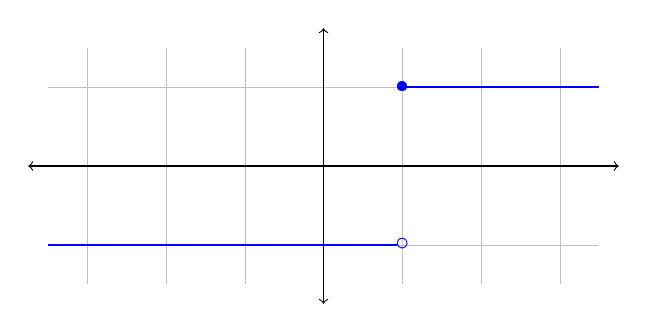
\begin{tikzpicture}
	  \draw[ultra thin,color=lightgray] (-3.5,-1.5) grid (3.5,1.5);   % coordinate grid
	  \draw[<->] (-3.75,0) -- (3.75,0);% node[right] {$x$};   % x-axis
	  \draw[<->] (0,-1.75) -- (0,1.75);% node[above] {$y$};   % y-axis
	
	%   \foreach \x/\xtext in {-4,...,-1,1,2,3,4}        % x-axis labels
	%   \draw (\x,2pt) -- (\x,-2pt) node[anchor=north, font=\footnotesize] {$\xtext$}; 
	
	%   \foreach \y/\ytext in {-4,..., -1,1,2,3, 4}           % y-axis labels
	%   \draw (2pt,\y) -- (-2pt,\y) node[anchor=east, font=\footnotesize] {$\ytext$}; 
	
	  % parametric function alpha(t)
	%   \draw [thick, samples=100,smooth] plot[variable=\t, domain=0:2*pi] ({3*cos(\t r)^3},{3*sin(\t r)^3});

	\draw [thick, samples=100,smooth, color=blue] plot[variable=\t, domain=-3.5:0.935] ({\t, -1});
	\draw [thick, samples=100,smooth, color=blue] plot[variable=\t, domain=1:3.5] ({\t, 1});

	\node at (1, -1) {\color{blue} $\circ$};
	\node at (1, 1) {\color{blue} \textbullet};
	
	\end{tikzpicture}
	\end{center}

	This function is not continuous at $1$. To see this, note that $1 - 1/n \rightarrow 1$ but $f(1 - 1/n) \rightarrow -1 \neq f(1)$ as $n \rightarrow \infty$.
\end{example}

\begin{example}[The Domain Matters]
Consider the function $f: \Q \rightarrow \R$ with
$$
\begin{cases}
	1 &\mbox{if } x^2 > 2, \\
	0 &\mbox{if } x^2 < 2.
   \end{cases}
$$
This function is continuous, since for every $a \in \Q$ there is an interval about $a$ for which $f$ is constant, so $f$ is continuous at $a$. If $f$ was defined on $\R$ instead of $\Q$, then it would be discontinuous only at $\pm\sqrt{2}$. But these points are not in our domain, so we don't need to worry about them.
\end{example}


\begin{example}[Continuity of $\sin 1/x$]\label{ex:sin-cont}
	Consider the function\footnote{I know that we haven't defined what $\sin$ is, but we will use it in examples because they are instructive. If this bothers you, feel free to come back after our discussion of power series.} $f: \R \rightarrow \R$ with $f(x) = \sin(1/x)$ if $x \neq 0$ and $f(0) = 0$.

	\begin{center}
		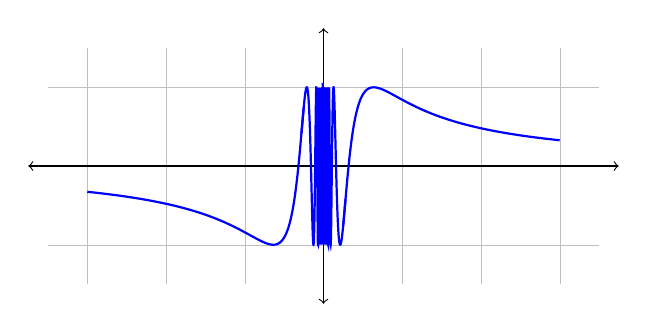
\begin{tikzpicture}
	  \draw[ultra thin,color=lightgray] (-3.5,-1.5) grid (3.5,1.5);   % coordinate grid
	  \draw[<->] (-3.75,0) -- (3.75,0);% node[right] {$x$};   % x-axis
	  \draw[<->] (0,-1.75) -- (0,1.75);% node[above] {$y$};   % y-axis
	
	%   \foreach \x/\xtext in {-4,...,-1,1,2,3,4}        % x-axis labels
	%   \draw (\x,2pt) -- (\x,-2pt) node[anchor=north, font=\footnotesize] {$\xtext$}; 
	
	%   \foreach \y/\ytext in {-4,..., -1,1,2,3, 4}           % y-axis labels
	%   \draw (2pt,\y) -- (-2pt,\y) node[anchor=east, font=\footnotesize] {$\ytext$}; 
	
	  % parametric function alpha(t)
	%   \draw [thick, samples=100,smooth] plot[variable=\t, domain=-3:3] (\t,sin(1/t));

	% \draw [thick, samples=100,smooth, color=blue] plot[variable=\t, domain=-3.5:0.935] ({\t, -1});
	% \draw [thick, samples=100,smooth, color=blue] plot[variable=\t, domain=1:3.5] ({\t, 1});

	\draw [thick, samples=100,smooth, color=blue] plot[variable=\t, domain=-3:-0.25] ({\t},{sin((\t)^(-1) r)});
	\draw [thick, samples=300,smooth, color=blue] plot[variable=\t, domain=-0.28:-0.005] ({\t},{sin((\t)^(-1) r)});
	\draw [thick, samples=300,smooth, color=blue] plot[variable=\t, domain=0.005:0.28] ({\t},{sin((\t)^(-1) r)});
	\draw [thick, samples=100,smooth, color=blue] plot[variable=\t, domain=0.25:3] ({\t},{sin((\t)^(-1) r)});
	% \draw [thick, samples=100,smooth] plot[variable=\t, domain=0.0001:3] (\t,{sin(1/t)});
	% \node at (1, -1) {\color{blue} $\circ$};
	% \node at (1, 1) {\color{blue} \textbullet};
	
	\end{tikzpicture}
	\end{center}
	This function is not continuous at $x = 0$. To see this, consider the sequence $a_n = \frac{1}{2\pi n + \pi/2}$. Then $a_n \rightarrow 0$, but $f(a_n) = 1 \rightarrow 1 \neq f(0)$ as $n \rightarrow \infty$.
\end{example}

\begin{example}[A Functional Equation with Continuity]
	We wish to find all continuous functions $f: \R \rightarrow \R$  such that $f(x) + f(2x) = 0$.

	Letting $x = 0$ we get $f(0) = 0$. Then rearranging we have
	$f(x) = -f(x/2)$, and repeatedly using this gives
	$$
	f(x) = -f\left(\frac{x}{2}\right) = f\left(\frac{x}{4}\right) = -f\left(\frac{x}{8}\right) = \cdots = (-1)^{n}f\left(\frac{x}{2^n}\right).
	$$
	Then since $f$ is continuous we have $f(x) = \lim_{n \to \infty} (-1)^n f(x/2^n) = f(0) = 0$. Thus $f(x) = 0$ is the only such function, which clearly works.
\end{example}


When attempting to determine if a function is continuous, one should keep in mind the following properties of continuity (all of which follow directly from our basic properties of limits).

\begin{proposition}[Sums, Products and Reciporicals of Continuous Functions]
	Let $f, g: A \rightarrow \C$ be functions. Then the following hold.
	\begin{enumerate}[label=(\roman*)]
		\item If $f$ and $g$ are continuous at $a$, then so is their sum $f + g$.
		\item If $f$ and $g$ are continuous at $a$, then so is their product $fg$.
		\item If $f$ is continuous at $a$ and $f(a) \neq 0$ then so is $1/f$.
	\end{enumerate}
\end{proposition}
\begin{proof}
	We prove each individually using the limit definition of continuity.
	\begin{enumerate}[label=(\roman*)]
		\item If $\displaystyle\lim_{z \to a} f(z) = f(a)$ and $\displaystyle\lim_{z \to a} g(z) = g(a)$ then $\displaystyle\lim_{z \to a} (f+g)(z) = (f+g)(a)$.
		\item If $\displaystyle\lim_{z \to a} f(z) = f(a)$ and $\displaystyle\lim_{z \to a} g(z) = g(a)$ then $\displaystyle\lim_{z \to a} (fg)(z) = (fg)(a)$.
		\item If $\displaystyle\lim_{z \to a} f(z) = f(a)$ and $f(a) \neq 0$, then $\displaystyle\lim_{z \to a} 1/f(z) = 1/f(a)$.
		 \qedhere
	\end{enumerate}
	% \begin{enumerate}[label=(\roman*)]
	% 	\item If $a_n \in A$ and $a_n \rightarrow a$, then $(f + g)(a_n) = f(a_n) + g(a_n) \rightarrow f(a) + g(a) = (f + g)(a)$ as $n \rightarrow \infty$. So $f + g$ is continuous at $a$.
	% 	\item If $a_n \in A$ and $a_n \rightarrow a$, then $(fg)(a_n) = f(a_n)g(a_n) \rightarrow f(a)g(a) = (fg)(a)$ as $n \rightarrow \infty$. So $fg$ is continuous at $a$.
	% 	\item If $a_n \rightarrow a$ and $f(a_n) \neq 0$ for all $n$, then $1/f(a_n) \rightarrow 1/f(a)$. So $1/f$ is continuous at $a$. \qedhere
	% \end{enumerate}
\end{proof}

Along with the fact that $f(x) = x$ and $f(x) = c$ are continuous, these properties imply that all polynomials are continuous.


\begin{proposition}[The Composition of Continuous Functions is Continuous]
	Let $f: A \rightarrow B$ and $g: B \rightarrow \C$ with $A, B \subseteq \C$. Then if $f$ is continuous at $a \in A$ and $g$ is continuous at $f(a)$, then $g \circ f$ is also continuous at $a$.
\end{proposition}
\begin{proof}
	If $a_n \rightarrow a$ then by the continuity of $f$ we have $f(a_n) \rightarrow f(a)$, and by the continuity of $g$ we have $g(f(a_n)) \rightarrow g(f(a))$. So $g\circ f$ is continuous at $a$.
\end{proof}

\subsection{The Intermediate Value Theorem}

Continuous functions are nice because they have a few nice properties. The first of these that we will prove is the \emph{intermediate value theorem}, a central theorem in elementary analysis. The idea of the intermediate value theorem is that if a continuous function starts at one value and ends at a different value, then it must take on all of the values in between.

\begin{center}
	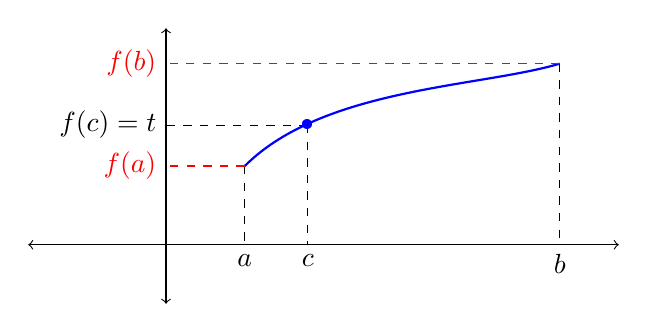
\begin{tikzpicture}
%   \draw[ultra thin,color=lightgray] (-3.5,-0.5) grid (3.5,2.5);   % coordinate grid
  \draw[<->] (-3.75,0) -- (3.75,0);% node[right] {$x$};   % x-axis
  \draw[<->] (-2,-0.75) -- (-2,2.75);% node[above] {$y$};   % y-axis

%   \foreach \x/\xtext in {-4,...,-1,1,2,3,4}        % x-axis labels
%   \draw (\x,2pt) -- (\x,-2pt) node[anchor=north, font=\footnotesize] {$\xtext$}; 

%   \foreach \y/\ytext in {-4,..., -1,1,2,3, 4}           % y-axis labels
%   \draw (2pt,\y) -- (-2pt,\y) node[anchor=east, font=\footnotesize] {$\ytext$}; 

  % parametric function alpha(t)
%   \draw [thick, samples=100,smooth] plot[variable=\t, domain=0:2*pi] ({3*cos(\t r)^3},{3*sin(\t r)^3});

% \draw [thick, samples=100,smooth, color=blue] plot[variable=\t, domain=-3.5:0.935] ({\t, -1});
% \draw [thick, samples=100,smooth, color=blue] plot[variable=\t, domain=1:3.5] ({\t, 1});

% \node at (0, 0) {\color{blue} $\textbullet$};


%Curve Lines [id:da5569099817019642] 
\draw[thick, smooth, color=blue]    (-1,1) .. controls (0,2) and (2,2) .. (3,2.3) ;

\draw  [dashed] (-1, 1) -- (-1, 0) node [below] {$a$};
% \node at (-1, 0) {$a$};
\draw  [dashed, ] (3, 2.3) -- (3, 0) node [below] {$b$};

\draw  [dashed, red] (3, 2.3) -- (-2, 2.3) node [left] {$f(b)$};
\draw  [dashed, red] (-1, 1) -- (-2, 1) node [left] {$f(a)$};
% \node at (3, 0) {$b$};

\draw  [dashed] (-0.2, 1.52) -- (-0.2, 0) node [below] {$c$};
\draw  [dashed] (-0.2, 1.52) -- (-2, 1.52) node [left] {$f(c)=t$};

\node at (-0.2, 1.52) {\color{blue}\small \textbullet};





\end{tikzpicture}
\end{center}

In the proof below we will employ suprema\footnote{If you are unfamiliar with this term and/or the least upper bound principle, feel free to have a look at Chapter 2 of my `Numbers and Sets' course notes.}, but we will give another proof afterwards that does not use this (at the expense of being slightly longer).

\begin{theorem}[The Intermediate Value Theorem]
	Let $f: [a, b] \rightarrow \R$ be a continuous function. Then for every $t$ between $f(a)$ and $f(b)$ there is an $c \in [a, b]$ with $f(c) = t$.
\end{theorem}
\begin{proof}
Suppose without loss of generality\footnote{If $t = f(a)$ or $t = f(b)$ then we are done. Also the case $f(a)> t> f(b)$ follows similarity.} that $f(a) < t < f(b)$. Consider the set $S = \{x \in [a, b] : f(x) < t\}$. This set is bounded and since $a \in S$ it is non-empty. So we can let $c = \sup S$, and note that $a \leq c \leq b$.

Let $n \geq 1$ be an integer. Then since $c$ is the supremum there must exist some $x_n \in S$ such that $c - \frac{1}{n} < x_n \leq c$. 
By the squeeze theorem we have $x_n \rightarrow c$ as $n \rightarrow \infty$.
Also $f$ is continuous so $f(x_n) \rightarrow f(c)$. 
We also constructed $x_n$ to be in $S$, giving $f(x_n) < t$ for all $n$. This implies that $f(c) \leq t$. 

We know that $c \in [a, b]$ but $c \neq b$, so there is some integer $N$ such that for $n \geq N$ we have $c + 1/n \leq b$.
Using that $c$ is the supremum, we have $c + 1/n \not \in S$ for all $n \geq N$, that is, $f(c + 1/n) \geq t$ for all $n\geq N$.
Then by continuity we have $f(c) \geq t$. 

But then $f(c) \geq t$ and $f(c) \leq t$, so we must have $f(c) = t$.
\end{proof}

Before we look at some examples of using the intermediate value theorem, there's a few things worth noting about the intermediate value theorem.

First of all, we say absolutely nothing about uniqueness in the theorem. It is very much possible for a function to take on an intermediate value multiple times.
Second of all, when applying the intermediate value theorem (commonly abbreviated to IVT) a good general problem solving technique is trying to apply IVT to other related functions such as $g(x) = f(x) - x$ or $g(x) = f(x) - t$ and things like that. You will see this `trick' show up in the examples below, and also again when we get to Rolle's theorem and the mean value theorem.


\begin{example}[Fixed Points of Continuous Maps from ${[0,1]}$ to Itself]
	We will prove that if $f:[0, 1] \rightarrow [0, 1]$ is a continuous function then there is some $c \in [0, 1]$ such that $f(c)=c$.

	Consider the function $g(x) = f(x) - x$. Then $g$ is continuous with $g(0) = f(0)$ and $g(1) = f(1) - 1$. 
	Since $0 \leq f(x) \leq 1$, we must have $g(0) \geq 0$ and $g(1) \leq 0$. Thus by the intermediate value theorem there exists some $c \in [0, 1]$ such that $g(c) = 0$. But then we have $f(c) - c = 0$, that is, $f(c) = c$ as required.
\end{example}

\begin{example}[Existence $n$th Roots]
	We will show that for any positive integer $n$ and $y > 0$ there exists a real number $x$ such that $x^n = y$.

	Consider the function $f(x) = x^n$. This function is continuous on $[0, 1 + y]$, and since $f(0) = 0$ and $f(1 + y) = (1 + y)^n$, we have $f(0) < y < f(1 + y)$.
	Thus by the intermediate value theorem there is some $x \in [0, 1+ y]$ such that $f(x) = y$, that is, $x^N = y$.
\end{example}

Now before we look on let's have a look at an alternative proof for the intermediate value theorem. This proof uses the same idea as the previous proof (try to see why) but avoids the use of suprema.

\begin{aside}{Aside: Hunting For \st{Lions} Intermediate Values}
	It was mentioned before that the `lion hunting' technique that we used to prove the Bolzano–Weierstrass theorem could also be used to prove other theorems in Analysis. One such example is the intermediate value theorem.

	The steps in the proof are quite similar to that of the proof of the Bolzano-Weierstrass theorem, the only difference is what we are `hunting for', which in this case is our intermediate value, and how we finish off the proof.

	\begin{proof}[Proof (Intermediate Value Theorem, Lion Hunting Style)]
Again suppose without loss of generality that $f(a) < t < f(b)$.
We are going to define two sequences $a_n$ and $b_n$ inductively as follows. Begin by setting $a_1 = a$ and $b_1=b$, and let $c = (a_1 + b_1)/2$ be the midpoint $a_1$ and $b_1$.

Then there is two possibilities:
\begin{enumerate}
\item $f(c_1) \geq t$.
\item $f(c_1) < t$.
\end{enumerate}
If the first one holds, we set $a_2 = a_1$ and $b_2 = c_1$, and if it doesn't then we set $a_2 = c_1$ and $b_2 = b_1$.
Repeating this process, we construct $a_n$ and $b_n$ such that $f(a_n) \leq t \leq f(b_n)$, $a_{n - 1} \leq a_n \leq b_n \leq b_{n - 1}$, and also $b_n - a_n = (b_{n - 1} - a_{n - 1})/2$.

Now $a_n$ is increasing and bounded above, and $b_n$ is decreasing and bounded below and thus $a_n \rightarrow c \in [a, b]$, and $b_n \rightarrow c' \in [a, b]$. Then we have $c - c' = (c - c')/2$ using the above result, and thus $c = c'$.

Since $f$ is continuous at $c$ and $a_n \rightarrow c$, we know that $f(a_n) \rightarrow c$ as $n \rightarrow \infty$. Since $f(a_n) \leq t$, we also know that $f(c) \leq t$. Similarity we also have $f(b_n) \geq t$, so $f(c) \geq t$. But then $t \leq f(c) \leq t$, and thus $f(c) = t$, and we are done.
	\end{proof}

	To get a feel for the construction, try drawing a rough sketch of the process. If you consider the case of a function that takes on the desired intermediate value multiple times, you should also see the that this proof does not give the same value for $c$ as the previous proof.

\end{aside}


A natural question upon learning of the intermediate value theorem is if it is equivalent to definition of continuity. The answer to this question is no -- there are functions that have the `intermediate value property', without being continuous. One example is $\sin(1/x)$ which we showed is discontinuous at $x = 0$ in \autoref{ex:sin-cont}. Another more elaborate example is `Conway's Base-13 Function', which has the intermediate value property but is discontinuous everywhere. You can read more about this function on \href{https://en.wikipedia.org/wiki/Conway_base_13_function}{Wikipedia}.


\subsection{The Boundedness Theorem}

The last result about continuous functions that we will prove is the \emph{boundedness theorem}, another central theorem in elementary analysis. The statement of this result is straightforward: a continuous function on a closed bounded interval is bounded and attains its bounds.

First we will prove that a continuous function defined on some closed interval is indeed bounded.
\begin{lemma}[Continuous Function on Closed Interval is Bounded]
	If $f:[a, b] \rightarrow \R$ is continuous then there exists $K$ such that $|f(x)| \leq K$ for all $x \in [a, b]$.
\end{lemma}
\begin{proof}
If $f$ was unbounded, then given any integer $n \geq 1$ there exists $x_n \in [a, b]$ such that $|f(x_n)| > n$. By Bolzano–Weierstrass, $x_n$ has a convergent subsequence $x_{n_j} \rightarrow x$. Also since $a \leq x \leq b$, we must have $x \in [a, b]$.
By continuity of $f$, $f(x_{n_j}) \rightarrow f(x)$, but $|f(x_{n_j})| > n_j$, and thus does not tend to a limit. Thus we have a contradiction.
\end{proof}

Now we can prove that such a continuous function attains its bounds, giving us the boundedness theorem.

\begin{theorem}[Boundedness Theorem]
	If $f:[a, b] \rightarrow \R$ is continuous then there exists $x_1, x_2 \in [a, b]$ such that $f(x_1) \leq f(x) \leq f(x_2)$ for all $x \in [a, b]$.
\end{theorem}
\begin{proof}
	By our previous lemma, we know that $f$ is bounded. Now we define the set
	$$
	A = \{f(x) : x \in [a, b]\}.
	$$
	This set is bounded and non-empty and thus has a supremum $M = \sup A$. Then for each positive integer $n$, $M - 1/n$ cannot be an upper bound for $A$. This implies that there is some $x_n \in [a, b]$ such that $M - 1/n < f(x_n) \leq M$.

	By Bolzano–Weierstrass, $x_n$ has a convergent subsequence $x_{n_j} \rightarrow x$. Since $a \leq x_n \leq b$, we know $a \leq x \leq b$. By the continuity of $f$, $f(x_{n_j}) \rightarrow f(x)$, but $f(x_{n_j}) \rightarrow M$ by construction. 
	So $f(x) = M$. So $x_2 = x$. The minimum follows analogously. \qedhere

	\emph{Alternate Proof}. As before, let $M = \sup A$ and suppose that there was no $x_2$ such that $f(x_2) = M$. Then let $g(x) = \frac{1}{M - f(x)}$ for $x \in [a, b]$. This function is well defined and continuous. Now $g$ must be bounded by the previous lemma, so $g(x) \leq K$ for all $x \in [a, b]$, for some $K$. This means that $f(x) \leq M - 1/k$ on $[a, b]$. This is contradiction since we set $M$ as the supremum. \hfill\qed
\end{proof}

\clearpage
\section{Differentiability}

You are likely familiar with differentiability (and particularly the computation of derivatives) from calculus. While this knowledge should certainly not be disregarded, we are going to go from the beginning, doing everything with a little more care than it got in calculus.
Throughout this section we will deal with functions $f: A \subseteq \R \rightarrow \R$,
though the basic definitions will apply to $\C$.\footnote{We will use differentiation over $\C$ in our discussion of power series though. One should also note that the other basic rules such as the sum, product and chain rules will also hold over $\C$, but being differentiable over $\C$ is a stronger condition than being differentiable over $\R$ or $\R^2$. For example, consider $f(z) = \overline{z}$, which is not complex differentiable.}.

Here's our basic definition:

\begin{definition}[Differentiability]
	Let $A \subseteq \R$ and $f: A \rightarrow \R$. 
	Then if $x$ is a limit point of $A$, we say that $f$ is \vocab{differentiable at $x$} with derivative $f'(x)$ if
	$$
	\lim_{h \to 0} \frac{f(x + h) - f(x)}{h} = f'(x).
	$$

	We say that $f$ is \vocab{differentiable} on $A$ if $f$ is differentiable at every $x \in A$.
\end{definition}

Let's pause for a moment. The core idea of differentiation is 
we want to \emph{approximate a function around some point using a linear map}\footnote{Indeed it is which this idea, not really that of `the tangent to a curve' that is used to generalise the derivative to functions of multiple variables. Of course they are closely related.}. Indeed, our definition of the derivative is directly equivalent to the following: $f$ is differentiable at $x$ if
$$
	f(x + h) = f(x) + f'(x)h + \varepsilon(h),
$$
where $\lim_{h\to 0} \varepsilon(h)/h = 0$. That is, it is differentiable if we can approximate the function with some linear map where the error decreases faster than linearly.


% \begin{remark}[Notation]
% 	It is common to write $f'(x) = \frac{\mathrm{d} y}{\mathrm{d} x} = \frac{\mathrm{d} f}{\mathrm{d} x}$, all of which work equally well.
% \end{remark}

\subsection{Properties of Differentiable Functions}

With that spiel over, we can move on to some properties of differentiable functions. The first is that differentiability implies continuity.

\begin{proposition}[Differentiability Implies Continuity]
	If $f$ is differentiable at $x$, then $f$ is continuous at $x$.
\end{proposition}
\begin{proof}
	Using the limit definition of continuity we have
	$$\lim_{h \to 0} \left[f(x + h) - f(x)\right] = \lim_{h \to 0} \frac{f(x + h) - f(x)}{h} \cdot (h) = f'(x) \cdot 0 = 0,
	$$
	thus $\lim_{h \to 0} f(x + h) = f(x)$, so $f$ is continuous at $x$.
\end{proof}

Now we can prove some basic rules for computing derivatives.

\begin{proposition}[Sum, Produt \& Quotient Rules]
	Suppose that $f: \R \rightarrow \R$ and $g: \R \rightarrow \R$ are differentiable at $x$ with derivatives $f'(x)$ and $g'(x)$.
	Then the following hold.
	\begin{enumerate}[label=(\roman*)]
		\item $f + g$ is differentiable at $x$, with $(f + g)'(x)= f'(x) + g'(x)$,
		\item $fg$ is differentiable at $x$, with $(fg)'(x) = f'(x)g(x) + f(x)g'(x)$,
		\item If $g'(x) \neq 0$ then $f/g$ is differentiable at $x$, with $(f/g)'(x) = \frac{g(x)f'(x) - g'(x)f(x)}{g^2(x)}$.
	\end{enumerate}
\end{proposition}
\begin{proof}
	We prove each individually.
	\begin{enumerate}[label=(\roman*)]
		\item This follows from the sum of limits.
		\item We have by the continuity of $f$
		\begin{align*}
			&\lim_{h \to 0} \frac{f(x + h)g(x + h) - f(x)g(x)}{h} \\
			=\ &\lim_{h \to 0}\left[ f(x+h) \frac{g(x + h) - g(x)}{h} + g(x)\frac{f(x + h) - f(x)}{h}\right],
		\end{align*}
		and by the continuity of $f$ and $g$ at $x$ we have $(fg)'(x) = f(x)g'(x) + f'(x) g(x)$.
		\item Similarly we have
		\begin{align*}
			&\lim_{h \to 0} \frac{f(x + h)/g(x + h) - f(x)/g(x)}{h} \\
		=\ &\lim_{h \to 0} \frac{1}{g(x)g(x + h)} \left[g(x)\frac{f(x + h) - f(x)}{h} - f(x) \frac{g(x + h) - g(x)}{h}\right],
		\end{align*}
		and by the continuity of $f$ and $g$ we have $(f/g)'(x) = \frac{g(x)f'(x) - g'(x)f(x)}{g^2(x)}$. \qedhere
	\end{enumerate}
\end{proof}


We will now prove the chain rule, which tells us how to compute the derivative of the composition of functions. Unfortunately this proof is quite `tricky', and trying to do something like we did in the proof above will not work. Instead, we need to return to our equivalent definition of differentiability, with $f(x + h) = f(x) + f'(x) h + \varepsilon(h)$, where $\displaystyle\lim_{h \to 0}\varepsilon(h)/h = 0$.

\begin{proposition}[Chain Rule]
	Suppose $f: \R \rightarrow \R$ is differentiable at $x$ and $g: \R \rightarrow \R$ is differentiability at $f(x)$. Then $g \circ f$ is differentiable at $x$ with $(g \circ f)'(x) = g'(f(x)) \cdot f'(x)$.
\end{proposition}
\begin{proof}
	We have
	\begin{align*}
	f(x + h) &= f(x) + f'(x)h + \varepsilon_f(h) \\
		g(f(x) + h) &= g(f(x)) + g'(f(x)) h + \varepsilon_g(h),
	\end{align*}
	where $\varepsilon_f(h)/h, \varepsilon_g(h)/h \rightarrow 0$ as $h \rightarrow 0$. From this we obtain
	\begin{align*}
		g(f(x + h)) &= g(f(x) + f'(x)h + \varepsilon_f(h)) \\
		&= g(f(x)) + g'(f(x))(f'(x)h + \varepsilon_f(h)) + \varepsilon_g(f'(x)h + \varepsilon_f(h)).
	\end{align*}
	Rearranging we get
	\begin{align*}
		&\lim_{h \to 0}\frac{g(f(x + h)) - g(f(x))}{h}\\
		=\ &\lim_{h \to 0} \frac{g'(f(x))(f'(x)h + \varepsilon_f(h)) + \varepsilon_g(f'(x)h + \varepsilon_f(h))}{h} \\
		=\ &g'(f(x))f'(x) +  \lim_{h \to 0}g'(f(x)) \frac{\varepsilon_f(h)}{h} +\lim_{h \to 0}\frac{\varepsilon_g(f'(x)h + \varepsilon_f(h))}{h}.
	\end{align*}
	Then as $h \rightarrow 0$ we have $\varepsilon_f (h)/h \rightarrow 0$ and $f'(x)h + \varepsilon_f(h) \rightarrow 0$ so $\varepsilon_g(f'(x)h + \varepsilon_f(h))/h \rightarrow 0$, and thus we have
	$
	(g \circ f)'(x) = g'(f(x))f'(x).
	$
\end{proof}


% Let's finish this subsection by looking at some examples of computing derivatives.

\begin{example}[Using the Chain Rule]
	Let $f(x) = \sin(x^2)$. Then since $(\sin x)' = \cos x$ we have $f'(x) = 2x \cos (x^2)$.
\end{example}
\begin{example}[A Continuous Everywhere But Non-Differentiable Function]
	Consider the function $f(x) = x \sin(1/x)$ when $x \neq 0$, and $f(0) = 0$. This function is continuous everywhere\footnote{Feel free to check this!}, but we will show that it is not differentiable at $x = 0$.

	At $x \neq 0$ this is differentiable by the chain rule, but at $x = 0$ we would need the following limit to exist:
	$$
	\lim_{h \to 0} \frac{(0 + h)\sin\left(\frac{1}{x + h}\right) - 0\sin\left(\frac{1}{x}\right)}{h} = \lim_{h \to 0} \sin\left(\frac{1}{h}\right),
	$$
	but this limit does not exist (a similar construction to \autoref{ex:sin-cont} will show this), and thus $f$ is not differentiable at $x = 0$.
\end{example}

Now in the example above we have a continuous everywhere function that's not differentiable at $0$. A related example is one of a function that is differentiable everywhere (and hence continuous), but whose derivative is discontinuous.

\begin{example}[A Function with Discontinuous Derivative]
	Consider the function $f(x) = x^2 \sin(1/x)$ when $x \neq 0$ and $f(0) = 0$.

	For $x \neq 0$ we have that $f$ is differentiable by the chain rule, and the derivative is given by
	$$
	f'(x) = x\sin\left(\frac{1}{x}\right) + \cos\left(\frac{1}{x}\right).
	$$

	For $x = 0$, we compute the derivative directly. We have
	$$
	f'(0) = \lim_{h \to 0} \frac{f(0 + h) - f(0)}{h} = \lim_{h \to 0} \frac{h^2\sin\left(\frac{1}{h}\right)}{h} = 0.
	$$

	Thus we can see that $f'$ is not continuous, since $f'(x) \not \rightarrow 0$ as $x \rightarrow 0$ (as $\cos 1/x$ is not continuous).

	\begin{center}
		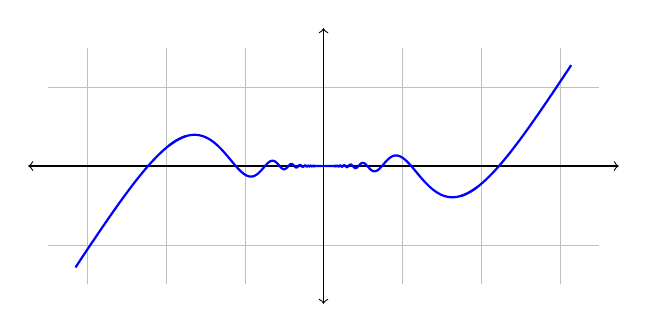
\begin{tikzpicture}
	  \draw[ultra thin,color=lightgray] (-3.5,-1.5) grid (3.5,1.5);   % coordinate grid
	  \draw[<->] (-3.75,0) -- (3.75,0);% node[right] {$x$};   % x-axis
	  \draw[<->] (0,-1.75) -- (0,1.75);% node[above] {$y$};   % y-axis
	
	%   \foreach \x/\xtext in {-4,...,-1,1,2,3,4}        % x-axis labels
	%   \draw (\x,2pt) -- (\x,-2pt) node[anchor=north, font=\footnotesize] {$\xtext$}; 
	
	%   \foreach \y/\ytext in {-4,..., -1,1,2,3, 4}           % y-axis labels
	%   \draw (2pt,\y) -- (-2pt,\y) node[anchor=east, font=\footnotesize] {$\ytext$}; 
	
	  % parametric function alpha(t)
	%   \draw [thick, samples=100,smooth] plot[variable=\t, domain=-3:3] (\t,sin(1/t));

	% \draw [thick, samples=100,smooth, color=blue] plot[variable=\t, domain=-3.5:0.935] ({\t, -1});
	% \draw [thick, samples=100,smooth, color=blue] plot[variable=\t, domain=1:3.5] ({\t, 1});

	\draw [thick, samples=100,smooth, color=blue] plot[variable=\t, domain=-0.45:-0.25] ({7*\t},{8*(\t)^2 * sin((\t)^(-1) r)});
	\draw [thick, samples=300,smooth, color=blue] plot[variable=\t, domain=-0.28:-0.004] ({7*\t},{8*(\t)^2 * sin((\t)^(-1) r)});
	\draw [thick, samples=300,smooth, color=blue] plot[variable=\t, domain=0.004:0.28] ({7*\t},{8*(\t)^2 * sin((\t)^(-1) r)});
	\draw [thick, samples=300,smooth, color=blue] plot[variable=\t, domain=-0.0045:0.0045] ({7*\t},{0});
	\draw [thick, samples=100,smooth, color=blue] plot[variable=\t, domain=0.25:0.45] ({7*\t},{8*(\t)^2 * sin((\t)^(-1) r)});
	% \draw [thick, samples=100,smooth] plot[variable=\t, domain=0.0001:3] (\t,{\t^2 * sin(1/\t)});
	% \node at (1, -1) {\color{blue} $\circ$};
	% \node at (1, 1) {\color{blue} \textbullet};
	
	\end{tikzpicture}
	\end{center}
\end{example}

There is however a limit as to how discontinuous a derivative can be. In particular the derivative of a differentiable function must have the intermediate value property.

\begin{theorem}[Darboux's Theorem]
	If $f: \R \rightarrow \R$ is differentiable then $f'$ has the intermediate value property. That is to say, if $a < b$ and $f'(a) < z < f'(b)$ then there exists $c \in (a, b)$ with $f'(c) = z$.
\end{theorem}
\begin{proof}
Given $a<b$ and $z \in \mathbb{R}$ such that $f^{\prime}(a)<z<f^{\prime}(b)$, we wish to show there exists $c \in(a, b)$ such that $f(c)=z$. We can rewrite the condition as $f^{\prime}(a)-z<0<f^{\prime}(b)-z$. Now define $g(x)=f(x)-z x,$ and note that we have $g^{\prime}(a)<0<g^{\prime}(b)$.

We want to find $c \in(a, b)$ such that $g^{\prime}(c)=0$. Now, $g$ is continuous (since $f$ is continuous), and thus is bounded on $[a, b]$, and the minimum is attained say at some point $k$. We can't have $k=a$, as that would imply that $g^{\prime}(a) \geq 0,$ and we also can't have $k=b$ as that would imply $g^{\prime}(b) \leq 0$. Thus $k \in(a, b),$ and we must then have $g^{\prime}(k)=0,$ and we are done.
\end{proof}

\subsection{Rolle's Theorem \& The Mean Value Theorem}

The sign of a function's derivative at a point can tell us quite a bit about the behaviour of that function near that point.
In particular, knowing that the derivative at a point vanishes can be quite useful;.

\begin{definition}[Local Maxima \& Minima]
	Let $f: \R \rightarrow \R$. If there exists $\delta$ such that $|x - x_0| < \delta$ implies that $f(x_0) \leq f(x)$, then we call $x$ a \vocab{local maximum}. 
	Similarly if this implies that $f(x_0) \geq f(x)$, we call $x$ a \vocab{local minimum}. 
\end{definition}

Our important result is as follows:

\begin{lemma}[Derivative of Maxima]\label{lemma:maxima}
	Let $f: \R \rightarrow \R$. If $x$ is a local maximum or minimum of $f$ and $f$ is differentiable at $x$ then $f'(x) = 0$.
\end{lemma}
\begin{proof}
	Without loss of generality, assume that $x$ is a local maximum. Then there exists $\delta$ such that $|h| < \delta_1$ implies that $f(x + h) \leq f(x)$. 
	
	Then if $0 < h < \delta$ we have
	$$
		\frac{f(x + h) - f(x)}{h} \geq 0,
	$$
	and thus we have $f'(x) \geq 0$.

	Similarly if $- \delta < h < 0$ we have
	$$
	\frac{f(x + h) - f(x)}{h} \leq 0,
	$$
	and thus we have $f'(x) \leq 0$. Hence $f'(x) = 0$.
\end{proof}

When we combine this result with the boundedness theorem from our discussion about continuity, we end up with \emph{Rolle's theorem}.

\begin{theorem}[Rolle's Theorem]
	Let $f: [a, b] \rightarrow \R$ be a continuous function which is differentiable on $(a, b)$. Then if $f(a) = f(b)$ then there exists $c \in (a, b)$ such that $f'(c) = 0$.
\end{theorem}
\begin{proof}
	Since $f$ is differentiable, it is also continuous and thus by the boundedness theorem $f$ is bounded on $[a, b]$ and these bounds are achieved.
	Thus we can let $M = \max_{x \in [a, b]} f(x)$ and $m = \min_{x \in [a, b]} f(x)$.

	If $M = m$, then $f$ must be constant and $f'(x) = 0$ for all $x \in (a, b)$, so we are done.
	Otherwise $M > f(a)$ or $m < f(a)$. If $M > f(a)$ then since the bounds are attained there exists $c \in (a, b)$ such that $f(c) = M$. But them $M$ is a maximum, so by our previous lemma we have $f'(c) = 0$. A similar argument works if $m < f(a)$.
\end{proof}

A direct consequence of Rolle's theorem\footnote{It's possible to establish this theorem without Rolle's theorem, and then Rolle's theorem pops out as a special case. The proof is (more or less) just what we did for Rolle's theorem laid out explicitly in the proof of this theorem.} 
is another classic theorem of analysis, the \emph{mean value theorem}, which is frequently abbreviated to MVT.

\begin{theorem}[The Mean Value Theorem]
	Let $f: [a, b] \rightarrow \R$ be a continuous function which is differentiable on $(a, b)$. Then there exists $c \in (a, b)$ such that $f(b) - f(a) = f'(c)(b - a)$.
\end{theorem}
\begin{proof}
	Let $k = \frac{f(a) - f(b)}{a - b}$, and define $\phi(x) = f(x) - kx$. Note that $\phi(a) = \phi(b)$. Then by Rolle's theorem there exists $c \in (a, b)$ such that $\phi'(c) = 0$, that is $f'(c) = k$.
\end{proof}

The mean value theorem says something notable: the size of the derivative controls the size of the function, or (in rougher terms) it puts a restriction on know `badly behaved' the function can be.
Also, if we appeal to geometric intuition (as we have tried not to, it's an easy way to go wrong) we can see that the mean value theorem says, as R. P. Burn wrote in \emph{Numbers and functions}, ``for the graph of a differentiable function, there is always a tangent parallel to the chord''. Of course, we will quickly move on from geometrical thinking.\footnote{I guess here is a good place to mention how we can reason geometrically in analysis. Drawing pictures and thinking geometrically is a great way to understand how things work, to come up with counterexamples and much more. Still it is important to remember that \emph{basically nothing in this course is provable by appealing to geometric intuition.} Instead this type of thinking should just inform the `analysis' side of us how to approach things.} 

Now let's think about applying the mean value theorem to two different functions. Suppose that $f, g : [a, b] \rightarrow \R$ is continuous and differentiable on $(a, b)$, and $g(a) \neq g(b)$. Then the mean value theorem gives us $s, t \in (a, b)$ such that
$$
	\frac{f(b) - f(a)}{g(b) - g(a)} = \frac{(b - a)f'(s)}{(b - a)g'(t)} = \frac{f'(s)}{g'(t)}.
$$
A stronger version of the mean value theorem says that we can take $s = t$.

\begin{theorem}[Cauchy's Mean Value Theorem]
	Let $f, g : [a, b] \rightarrow \R$ be continuous functions which are differentiable on $(a, b)$. Then there exists $c \in (a, b)$ such that
	$$
	(f(b) - f(a))g'(c) = f'(c)(g(b) - g(a)).
	$$
\end{theorem}
\begin{proof}
	We define the function
	\begin{align*}
		\phi(x) &= \begin{vmatrix}
			1 & 1 & 1 \\
			f(a) & f(x) & f(b) \\
			g(a) & g(x) & g(b)
			\end{vmatrix}  \\
		&= \left[f(x)g(b) - f(b)g(x)\right] - [f(a)g(b) - f(b) g(a)] + [f(a) g(x) - f(x) g(a)].
	\end{align*}
	Then $\phi$ is continuous on $[a, b]$ and differentiable on $(a, b)$\footnote{If the use of determinants bothers you, then feel free to just look at the expansion. If also remember how integrals work, you can obtain $\phi$ from working backwards from what we need to arrive at.}. Also $\phi(a) =\phi(b) = 0$. Then by Rolle's theorem, there exists $c \in (a, b)$ such that $\phi'(c) = 0$.
	
	Differentiating $\phi$ we then have 
	$$
	\phi'(x) = f'(x)[g(b) - g(a)] + g'(x)[f(a) - f(b)],
	$$
	and thus $\phi'(c) = 0$ gives the desired result.
\end{proof}

Cauchy's mean value theorem has many applications. For example, we can use the mean value theorem to establish L'Hôpital's rule for evaluating limits.

\begin{example}[L'Hôpitel's Rule]
	We wish to evaluate $\displaystyle \lim_{x \to 0} \frac{e^x - 1}{\sin x}$.

	By Cauchy's mean value theorem, there exist $c \in (0, x)$ such that
	$
	\frac{e^x - e^0}{\sin x - \sin 0} = \frac{e^c}{\cos c}.
	$
	Then $c \rightarrow 0$ as $x \rightarrow 0$, and thus we get
	$$
	\lim_{x \to 0} \frac{e^x - 1}{\sin x} = \lim_{c \to 0}\frac{e^c}{\cos c} = 1.
	$$
\end{example}

In more generality:

\begin{theorem}[L'Hôpital's Rule]
	Suppose $f, g :[a, b] \rightarrow \R$ are continuous and differentiable on $(a, b)$. Suppose that $f(a) = g(a) = 0$, that $g'(x)$ does not vanish near $a$ and $f'(x)/g'(x) \rightarrow \ell$ as $x \rightarrow a$. Then $f(x)/g(x) \rightarrow \ell$ as $x \rightarrow a$.
\end{theorem}
\begin{proof}
Since $g^{\prime}(x)$ does not vanish near $a$, we can suppose that $g^{\prime}(x) \neq 0$ for $x \in(a, b)$, as otherwise we could just consider the subinterval $\left(a, b^{\prime}\right),$ defined so that this is the case.

By Cauchy's mean value theorem we have
$$
\frac{f(x)}{g(x)}=\frac{f(x)-f(a)}{g(x)-g(a)}=\frac{f^{\prime}(c)}{g^{\prime}(c)}
$$
where $c \in(a, x)$. Then $c \rightarrow a$ as $x \rightarrow a$, and hence $f(x) / g(x) \rightarrow \ell$ as $x \rightarrow a$.
\end{proof}

The mean value theorem can also help us extend \autoref{lemma:maxima}. Knowing the sign of a derivative over some interval can tell us immediately if it is constant, increasing or decreasing.

\begin{proposition}[Sign of the Derivative]\label{prop:sign}
	Let $f: [a, b] \rightarrow \R$ be differentiable on $(a, b)$. Then the following hold.
	\begin{enumerate}[label=(\roman*)]
		\item If $f'(x) \geq 0$ for all $x \in (a, b)$, then $f$ is monotonically increasing.
		\item If $f'(x) = 0$ for all $x \in (a, b)$, then $f$ is constant.
		\item If $f'(x) \leq 0$ for all $x \in (a, b)$, then $f$ is monotonically decreasing.
	\end{enumerate}
\end{proposition}
\begin{proof}
	By the mean value theorem we have $f(x_2) - f(x_1) = (x_2 - x_1)f'(x)$ where $a < x_1 < x < x_2 < b$. Then all of the results follow by considering the sign of $f'(x)$.
\end{proof}

\subsection{Inverses of Functions}

Before we move to slightly more exciting material, there's a few things about inverses of functions that we need to get out of the way. The proofs below are straightforward but require some care (by which I mean you have to avoid messing up which letter means what).

First of all, if we know that a continuous function is strictly increasing\footnote{If a continuous function was not strictly increasing or strictly decreasing then we couldn't have a unique inverse.} then we can deduce that the function has an inverse that is continuous and strictly increasing also. A similar result holds for strictly decreasing functions.

\begin{theorem}[Continuous Inverse Theorem]
	Let $f:[a, b] \rightarrow \R$ be a continuous and strictly increasing function. Then if $c = f(a)$ and $d = f(b)$, $f:[a, b] \rightarrow [c, d]$ is bijective and the inverse $f^{-1}: [c, d] \rightarrow [a, b]$ is continuous and strictly increasing.
\end{theorem}
\begin{proof}
	As $f$ is strictly increasing, it is an injection. It is also a surjection since if $c < t < d$ then there exists $x \in (a, b)$ such that $f(x) = t$. Thus $f$ is a bijection, and has an inverse $f^{-1}$.

	Since $f$ is strictly increasing, we can write this as $x_1 < x_2 \iff f(x_1) < f(x_2)$, so letting $f(x_1) = y_1$ and $f(x_2) = y_2$ we have 
	$f^{-1}(y_1) < f^{-1}(y_2) \iff y_1 < y_2$. Thus $f^{-1}$ is also strictly increasing.
	
	Now we will show $f^{-1}$ is continuous at some $y \in [c, d]$.
	Given $\epsilon > 0$, 
	let $x = f^{-1}(y)$. If $x \neq a, b$, we can find $\delta$ such that
	$$
		f(x - \epsilon) \leq f(x) - \delta < f(x) < f(x) + \delta \leq f(x + \epsilon).
	$$
	But then $|z - y| < \delta$ implies that $x - \epsilon < f^{-1}(z) < x + \epsilon$, so $|f^{-1}(z) - f^{-1}(y)| < \epsilon$.
	Thus $f^{-1}$ is continuous on $(a, b)$

	Otherwise, if $x = a$ we have $f(x) < f(x + \epsilon)$. Then $|z - y| < f(x + \epsilon) - f(x)$ implies that $|f^{-1}(z) - f^{-1}(y)| < \epsilon$, so $f^{-1}$ is continuous at $c$. A similar argument shows that it is continuous at $d$.
\end{proof}

Now this \emph{is} the differentiability section, so we can also describe what the derivative of a differentiable function's inverse is. This result is known as the one variable \emph{inverse function theorem}.

\begin{theorem}[Inverse Function Theorem]
	Let $f:[a, b] \rightarrow \R$ be continuous, strictly increasing, and differentiable on $(a, b)$.
	Then let $f(a) = c$ and $f(b) = d$. Then $f:[a, b] \rightarrow [c, d]$ is a bijection, and $f^{-1}$ is differentiable on $(c, d)$, with
	$$
	(f^{-1})'(x) = \frac{1}{f'(f^{-1}(x))}.
	$$
\end{theorem}
\begin{proof}
	By our previous theorem, $f$ is a bijection and $f^{-1}$ is a continuous and strictly increasing function. Let $y = f(x)$, with $x \in (a, b)$. We wish to show that $g'(y) = 1/f'(x)$.

	Given $k \neq 0$, let $h$ be given by $y + k = f(x + h)$, that is, $f^{-1}(y + k) = x + h$, where $h \neq 0$. Then
	$$
	\frac{f^{-1}(y + k) - f^{-1}(y)}{k} = \frac{h}{f(x + h) - f(x)}.
	$$
	Then since $f'(x) > 0$ and $f^{-1}$ is continuous (so $h \rightarrow 0$ as $k \rightarrow 0$) we have $k \to 0$ 
	$$
	\lim_{k \to 0} \frac{f^{-1}(y + k) - f^{-1}(y)}{k} = \lim_{h \to 0} \frac{x + h - x}{f(x + h) - f(x)} = \frac{1}{f'(x)},
	$$
	as required.
\end{proof}

\subsection{Taylor's Theorem}

We are now going to think about functions where we can take derivatives a number of times (getting higher-order derivatives).
We will begin by looking at how we can get an analogue of Rolle's theorem for higher-order derivatives. I will apologise in advance that this discussion is a bit long, so feel free to just skip to Taylor's theorem.

The following generalisation will come directly from Rolle's theorem.
\begin{theorem}[Higher-Order Rolle's Theorem]
	Let $f$ be continuous and $n-1$-times differentiable on $[a, b]$ and also $n$-times differentiable on $(a, b)$. Then if $f(a) = f'(a) = f''(a) = \cdots = f^{(n - 1)}(a) = 0$ and $f(b) = 0$ then there is a $c \in (a, b)$ such that $f^{(n)}(c) = 0$.
\end{theorem}
\begin{proof}
	Since $f(a) = f(b)$, by Rolle's theorem there exists $c_1 \in (a, b)$ such that $f'(c_1) = 0$. Then since $f'(a) = f'(c_1) = 0$, we can use Rolle's theorem again to obtain $c_2 \in (a, c_1)$ such that $f''(c_2) = 0$. Continuing on like this we obtain a $c_{n} \in (a, b)$ such that $f^{(n)}(c_n) = 0$, as required.
\end{proof}

We can also attempt to get some sort of `higher-order' mean value theorem. Recall that our proof of the mean value theorem was more or less as follows:
\begin{quotation}\noindent
	\emph{Define the function $\phi(x) = f(x) - kx$, where we choose $k$ such that the conditions of Rolle's theorem are satisfied.
	Then apply Rolle's theorem to $\phi$.}
\end{quotation}
We can try and do the same with a more elaborate construction. We will do this in three steps.
\begin{enumerate}
	\item Construct a polynomial $P(x)$ such that $P(a) = f(a)$, $P'(a) = f'(a)$, and so on until $P^{(n - 1)}(a) = f^{(n - 1)}(a)$.
	\item Construct another polynomial\footnote{We can think of this as the `error correcting term', because it fixes the discrepancy between $f(b)$ and $P(b)$ while not ruining the previous construction.} $E(x)$ such that $E^{(r)}(a) = 0$ for $r = 0, 1, \dots, n - 1$, but with $E(b) = f(b) - P(b)$.
	\item Take $\phi(x) = f(x) - P(x) - E(x)$.
\end{enumerate}
If we construct $\phi(x)$ in this way, then we will have $\phi(a) = \phi'(a) = \cdots = \phi^{(n - 1)}(a) = 0$, and also $\phi(b) = 0$, so it will satisfy our higher-order Rolle's theorem.

\begin{aside}{Aside: Constructing Our Polynomials}

	While it is likely you have seen a construction for $P$ before, I'd like to take a minute to spell it out in detail because it has some nice ideas.

	To construct this polynomial, what we really need is some construction of a term which affects the value of the polynomial at a point $a$ if and only if we are considering a certain derivative. We can do this as follows:
	$$
		Q_{k}(x) = \frac{(x - a)^k}{k!}.
	$$
	We can then (by taking derivatives) find that the value of this term is
	$$
	Q_k^{(j)}(a) = \begin{cases}
        1 &\mbox{if } j = k, \\
        0 &\mbox{if } j \neq k
       \end{cases}
	$$
	With this we can immediately write down an explicit construction for $P(x)$.
	\begin{align*}
		P(x) &= \sum_{k = 0}^{n - 1} f^{(k)}(a) Q_k(x) = \sum_{k = 0}^{n - 1} \frac{f^{(k)}(a)}{k!}(x - a)^k \\
		&= f(a) + f'(a) (x - a) + \frac{f''(a)}{2} (x - a)^2 + \cdots + \frac{f^{(n - 1)(a)}}{(n - 1)!} (x - a)^{n - 1}.
	\end{align*}

	This polynomial is known as the \vocab{Taylor polynomial} of degree $n - 1$ for $f$ about $a$. 

	We can use the exact same method to construct $E(x)$. 
	We need to not affect the first $n - 1$ derivatives at $x = a$, so we will need to add some multiple of $Q_{n}(x)$. However, this time we care about the value of the undifferentiated term at $x = b$:
	$$
	Q_{n}(b) = \frac{(b - a)^n}{n!}.
	$$
	Since we want $E(b) = f(b) - P(b)$, if we are going to have $E(x) = \lambda Q_n(x)$ we are going to need
	\begin{align*}
		\lambda Q_{n}(b) &= \lambda \frac{(b - a)^n}{n!} = f(b) - P(b) \\
\implies \lambda &= \frac{[f(b) - P(b)] \cdot n!}{(b - a)^n}.
	\end{align*}
	And thus we get
	\begin{align*}
		E(x) &= \frac{[f(b) - P(b)] \cdot n!}{(b - a)^n} Q_n(x) \\
		&= \left[f(b) - P(b)\right]\left(\frac{x - a}{b - a}\right)^n.
	\end{align*}
\end{aside}

Now with the constructions as above, we can write down $\phi(x) = f(x) - P(x) - E(x)$.
Then since $\phi(x)$ satisfies all of the conditions of our higher-order Rolle's theorem, there exists $c \in (a, b)$ such that $\phi^{(n)}(c) = 0$. 

Taking the $n$th derivative, since $P$ is a degree $n - 1$ polynomial and thus has a zero derivative, we get
\begin{align*}
	\phi^{(n)}(c) &= f^{(n)}(c) - [f(b) - P(b)] \cdot \frac{n!}{(b - a)^n} = 0 \\
\implies f(b)  &= P(b) + \frac{f^{(n)}(c)}{n!}(b - a)^n.
\end{align*}
for some $c \in (a, b)$. 

This result is Taylor's theorem, specially Taylor's theorem with the Lagrange form of the remainder. For completeness, this proof is given in a standalone form below.

\begin{theorem}[Taylor's Theorem with Lagrange Remainder]
	Let $f$ be continuous and $(n - 1)-$times differentiable on $[a, b]$ and $n$-times differentiable on $(a, b)$. Then we have
	$$
	f(b) = f(a) + f'(a)(b - a) + \cdots + \frac{f^{(n - 1)}(a)}{(n - 1)!}(b - a)^{n - 1} + \frac{f^{(n)}(c)}{n!}(b - a)^n,
	$$
	for some $c \in (a, b)$.
\end{theorem}
\begin{proof}
	We define
	$$
	\phi(x) = f(x) - \sum_{k = 0}^{n - 1} \frac{f^{(k)}(a)}{k!}(x - a)^k - M \left(\frac{x - a}{b - a}\right)^n,
	$$
	where $M$ is chosen such that $\phi(a) = \phi(b) = 0$.
	Then differentiating we have $\phi(a) = \phi'(a) = \cdots = \phi^{(n - 1)}(a) = 0$. 

	Then since $\phi(a) = \phi(b)$, there exists $c_1 \in (a, b)$ such that $\phi'(c_1) = 0$. Similarity $\phi'(a) = \phi'(c_1) = 0$, and thus there exists $c_2 \in (a, c_1)$ such that $\phi''(c_2) = 0$. Continuing on in this way, we find a $c_{n}$ such that $\phi^{(n)}(c_n) = 0$, where $c_n \in (a, b)$. 

	Then differentiating again we have
	$$
	\phi^{(n)}(c) = f^{(n)}(c) - \frac{M \cdot n!}{(b - a)^n} = 0.
	$$
	Now we know that $M$ is such that $\phi(b) = 0$, so we get
	$$
	M = f(b) - \sum_{k = 0}^{n - 1}\frac{f^{(k)}(a)}{k!} (b - a)^n.
	$$
	Thus we have
	\begin{align*}
		f^{(n)}(c) &= \frac{M \cdot n!}{(b - a)^n} = \left(f(b) - \sum_{k = 0}^{n - 1}\frac{f^{(k)}(a)}{k!} (b - a)^n\right) \cdot \frac{n!}{(b - a)^n} \\
\implies f(b) &= f(a) + f'(a)(b - a) + \cdots + \frac{f^{(n - 1)}(a)}{(n - 1)!}(b - a)^{n - 1} + \frac{f^{(n)}(c)}{n!}(b - a)^n,
	\end{align*}
	where $c \in (a, b)$ as required.
\end{proof}


So we have Taylor's theorem (which in this case can be thought of as a higher-order mean value theorem), let's try and do something with it. One of the main uses of Taylor's theorem is in giving us an infinite series which converges to the value of our function. This involves considering the terms of the degree $n$ taylor polynomial for increasing values of $n$, as we shall see.

Doing this type of problem has two main steps.
\begin{enumerate}
	\item Write down Taylor's theorem for the case of the function being considered.
	\item Show that the error term tends to zero as $n$ goes to infinity.
\end{enumerate}
We see how this is done using a Tripos question from 2010 (so eh spoilers I guess).

\begin{example}[Using Taylor's Theorem -- Part IA, 2010 Paper 1, Q10]
\emph{Problem}. Suppose that $e: \mathbb{R} \rightarrow \mathbb{R}$ is a differentiable function such that $e(0)=1$ and $e^{\prime}(x)=e(x)$ for all $x \in \mathbb{R}$. Use Taylor's theorem with the remainder in Lagrange's form to prove that
$$
e(x)=\sum_{n \geqslant 0} \frac{x^{n}}{n !} \quad \text { for all } \quad x \in \mathbb{R}
$$
[No property of the exponential function may be assumed.]

\emph{Solution}. We begin by noting that $e(x)$ is infinitely differentiable, with $e^{(n)}(x) = e(x)$. Indeed this is true for $n = 1$, and then it follows by induction for all $n$. Thus Taylor's theorem with Lagrange Remainder holds for all $n \in \N$.

Thus for all $n \in \N$ we have (using $e^{(n)}(0) = 1$ and $e^{(n)}(c) = e(c)$)
$$
e(x) = \sum_{k = 0}^{n - 1}\frac{x^k}{k!} + \frac{e(c) x^n}{n!} 
$$
for some $c \in (0, x)$.
And thus it suffices to show that $\frac{e(c)x^n}{n!} \rightarrow 0$ as $n \rightarrow \infty$, since that would imply that $e(x) - \sum_{k = 0}^{n - 1} \frac{x^k}{k!} \rightarrow 0$ as $n \rightarrow \infty$.
Now $e(t)$ is differentiable and hence continuous on $[0, x]$, and thus is bounded. So it suffices to show that $x^n/n! \rightarrow 0$, which holds.

Thus
$$
e(x) = \sum_{n = 0}^{\infty} \frac{x^n}{n!},
$$
as required.
\end{example}


Now it is \emph{not} the case that the remainder term always goes to zero. A common counterexample is $f(x) = \exp(-1/x^2)$ for $x \neq 0$ with $f(0) = 0$.

\clearpage
\section{Power Series}

Following on from our discussion of infinite series in Chapter 2, we are going to discuss a particular type of infinite series known as a \emph{power series}. Throughout this section, we are going to work mostly in $\C$.

\begin{definition}[Complex Power Series]
	A \vocab{complex power series} is an infinite series of the form
	$$
		\sum_{n = 0}^{\infty} a_n z^n,
	$$
	where $z \in \C$ and $a_n \in \C$.
\end{definition}

In this section we will look at some properties of power series, and we will use them to (finally) define some functions that we have alluded to quite a bit.

\subsection{Radius of Convergence}

Before we develop the concept of the radius of convergence, we first need to develop a lemma about the convergence of power series. 

\begin{lemma}[Absolute Convergence of Power Series]
Suppose that $\sum_{n = 0}^{\infty} a_n z_0^n$ converges for some $z_0 \in \C$. Then $\sum_{n = 0}^{\infty} a_n z^n$ converges absolutely for all $z\in \C$ with $|z| < |z_0|$.
\end{lemma}
\begin{proof}
Since $\sum_{n = 0}^{\infty} a_n z_1^n$ converges, we have $a_n z_1^n \rightarrow 0$, implying this sequence is bounded.
Then there is some $K > 0$ such that $|a_n z_1^n| < K$ for all $n$.	

So if $|z| < |z_0|$, we have $|a_n z^n| \leq K \left|z/z_1\right|^n$. Since the geometric series $\sum_{n = 0}^{\infty} |z/z_1|^n$ converges, our result follows by comparison.
\end{proof}

With this lemma we can prove one of our key results in the study of power series, the existence of the \emph{radius of convergence}.

\begin{theorem}[Radius of Convergence]
	Suppose that $a_n \in \C$. Then either the power series $\sum_{n = 0}^\infty a_n z^n$ converges for all $z \in \C$, or there exists a real number $R$ with $R \geq 0$ such that
	\begin{enumerate}[label=(\roman*)]
		\item $\sum_{n =0}^\infty a_n z^n$ converges absolutely if $|z| < R$,
		\item $\sum_{n =0}^\infty a_n z^n$ diverges if $|z| > R$.
	\end{enumerate}
	We say that $R$ is the \vocab{radius of convergence} of the power series.
\end{theorem}
\begin{proof}
	If $\sum_{n = 0}^\infty a_n z^n$ converges for all $z \in \C$, then we are done. Otherwise, there must exist $z_1 \in \C$ such that $\sum_{n = 0}^{\infty} a_n z_1^n$ diverges. Then by our previous lemma the power series must diverge for all $z \in \C$ where $|z| > |z_1|$.

	Now define the set $S = \{|z| : \sum_{n = 0}^\infty a_n z^n \text{ converges}\}$. This set is bounded above by $|z_1|$, and is non-empty since the power series converges for $z = 0$. Thus it has a supremum, say $R = \sup S$. 

	Then by definition $\sum_{n = 0}^{\infty} a_n z^n$ diverges if $|z| > R$, and then suppose $|z| < R$. Then there must be some $z_0$ with $|z| < |z_0| < R$ such that the power series converges for $z_0$ (by the definition of the supremum again). Then by our previous lemma the power series converges absolutely for $z$.
\end{proof}

What's quite lovely is that when we are inside the radius of convergence, the power series converges absolutely! This means that we can avoid all of those issues with rearranging series that show up when things don't converge absolutely. This can be quite helpful when actually working with power series.

What's also quite nice is that we can employ all of those lovely results we developed in \autoref{sec:2} to find what the radius of convergence of a power series is.
Let's look at two lemmas that come from the ratio and root tests, which can give the radius of convergence. 

\begin{lemma}[The Ratio Test for Radius of Convergence]
	Let $\sum_{n = 0}^{\infty} a_n z^n$ be a power series with radius of convergence $R$.
	Then if $|a_{n + 1}/a_n| \rightarrow \ell$ as $n \rightarrow \infty$, we have $R = 1/\ell$ if $\ell \neq 0$, and convergence everywhere if $\ell = 0$.
\end{lemma}
\begin{proof}
	By the ratio test, we have absolute convergence if 
	$$
	\lim_{n \to \infty} \left|\frac{a_{n + 1}}{a_{n}} \cdot \frac{z^{n + 1}}{z^n}\right| < 1.
	$$
	So if $\ell = 0$, then we have convergence everywhere. Alternatively, if $|z| < 1/\ell$ we have absolute convergence, and if $|z| > 1/\ell$ the series diverges, again by the ratio test.
\end{proof}

\begin{lemma}[The Root Test for Radius of Convergence]
	Let $\sum_{n = 0}^{\infty} a_n z^n$ be a power series with radius of convergence $R$.
	Then if $|a_{n}|^{1/n} \rightarrow \ell$ as $n \rightarrow \infty$, we have $R = 1/\ell$.
\end{lemma}
\begin{proof}
	By the root test, we have absolute convergence if
	$$
	\lim_{n \to \infty} |a_n z^n|^{1/n} < 1.
	$$
	So if $\ell = 0$, then we have convergence everywhere. Alternatively, if $|z| < 1\ell$ we have absolute convergence, and if $|z| > 1/\ell$ the series diverges, again by the root test.
\end{proof}

Now it is time for an important conceptual point: if we have a power series with radius of convergence $R$, then this only specifies the convergence/divergence inside or outside the circle $|z| = R$ (the \emph{circle of convergence}). Specifically {\color{red} it says nothing about the behaviour on the circle.} To see this, we will look at a few examples\footnote{This should remind you of the deadly sin mentioned in \autoref{sec:2}, where the root or ratio test said nothing if the limit was 1.}.

\begin{example}[Convergence on $|z| = R$]
	Consider the following power series:
	$$
	\text{(i) }\sum_{n = 0}^{\infty} z^n, \quad \text{(ii) }\sum_{n = 1}^\infty \frac{z^n}{n}\quad \text{(iii) }\sum_{n = 1}^\infty \frac{z^n}{n^2}.
	$$
	All of these have a radius of convergence $R = 1$, however for $|z| = 1$ for each power series we have:
	\begin{enumerate}
		\item Divergence if $|z| = 1$.
		\item Convergence\footnote{Have a look at Example Sheet 1 for this result} if $|z| = 1$ with $z \neq 1$, and divergence if $z = 1$.
		\item Convergence if $|z| = 1$.
	\end{enumerate}
	Thus we can't say anything about the case $|z| = R$ and each case really has to be treated separately.
\end{example}

\subsection{Differentiating Power Series}

So things are generally quite nice inside the circle of convergence. One of the nice things we can do is differentiate! Even better, we can differentiate power series just like we do polynomials!
The following results you need to know (including the lemmas), but the proofs are not examinable (feel free to skip them).

We are going to show that the power series $\sum_{n = 0}^{\infty} a_n z^n$ with radius of convergence $R$ has the derivative $\sum_{n = 0}^{\infty} n a_n z^{n - 1}$, whenever $|z| < R$.
Before showing this, we will need a lemma which gives us that this second power series converges for $|z| < R$.


\begin{lemma}
	Let $f(z) = \sum_{n = 0}^{\infty} a_n z^n$ be a power series whose radius of convergence is $R$. 
	Then if $0 < r < R$, the power series $\sum_{n = 1}^{\infty} n |a_n|r^{n - 1}$ converges.
\end{lemma}
\begin{proof}
	Pick $w$ such that $r < |w| < R$. Then the power series $\sum_{n = 0}^{\infty} a_n w^n$ converges, so the terms $|a_n w^n|$ are bounded above by say $M$. Then we have
	$$
	n|a_n|r^n = n|a_n w^n| \frac{r^n}{|w|^n} \leq M n \frac{r^n}{|w|^n}.
	$$

	But then the series $\sum_{n = 1}^{\infty} Mn (r/|w|)^n$ converges by the ratio test, and thus by the comparison test $\sum_{n = 1}^{\infty} n |a_n| r^{n - 1}$ converges.
\end{proof}

Applying this lemma twice also gives us that the power series
$
\sum_{n = 2}^{\infty} n(n - 1) |a_n| r^{n - 2}
$
converges. We are now ready to prove our theorem about differentiating power series.


\begin{theorem}[Differentiating Power Series]
	Let $f(z) = \sum_{n = 0}^{\infty} a_n z^n$ be a power series whose radius of convergence is $R$. Then $f$ is differentiable at all points with $|z| < R$, and
	$
	f'(z) = \sum_{n = 0}^{\infty} n a_n z^{n - 1}.
	$
\end{theorem}
\begin{proof}
	Using the difference of powers factorisation, we have
	\begin{align*}
		\frac{f(z+h)-f(z)}{h}&=\sum_{n=0}^{\infty} a_{n} \frac{(z+h)^{n}-z^{n}}{h}\\&=\sum_{n=1}^{\infty} a_{n}\left[(z+h)^{n-1}+(z+h)^{n-2} z+\cdots+z^{n-1}\right].
	\end{align*}
	Then, since $\sum_{n = 1}^\infty n a_n z^{n - 1}$ converges by our lemma, we have
	\begin{align*}
		\frac{f(z+h)-f(z)}{h}-\sum_{n=1}^{\infty} n a_{n} z^{n-1} &= \sum_{n = 1}^{\infty} a_n \left(\sum_{j=0}^{n-1} z^{j}(z+h)^{n-1-j}-z^{n-1}\right) \\
		&= \sum_{n = 1}^{\infty} a_n \left(\sum_{j=0}^{n-1} z^{j}\left[(z+h)^{n-1-j}-z^{n-1 - j}\right]\right).
	\end{align*}
	Now we want to bound the terms of this inside sum. Choose $r$ such that $|z| < r < R$ and $h$ such that $|z| + |h| < r$. Then 
	employing the difference of powers factorisation again we get
	\begin{align*}
		|(z+h)^{n-1-j}-z^{n-1 - j}| &= |h((z + h)^{n - 2 - j} + z(z + h)^{n - 3 - j} + \cdots + z^{n - 2 - j})| \\
		&\leq |h|(n- 1 - j)r^{n - 2 - j}.
	\end{align*}
Applying this bound, assuming the right hand sum converges we have
\begin{align*}
	\left|\frac{f(z+h)-f(z)}{h}-\sum_{n=1}^{\infty} n a_{n} z^{n-1}\right| &\leq \sum_{n=1}^{\infty}\left|a_{n}\right|\left(\sum_{j=0}^{n-1} r^{j}|h|(n-1-j) r^{n-2-j}\right) \\
	&= |h| \sum_{n=1}^{\infty}\left|a_{n}\right| r^{n-2}\left(\sum_{j=0}^{n-1}j\right) \\
	&= \frac{1}{2}|h| \sum_{n=2}^{\infty}\left|a_{n}\right| n(n-1)r^{n-2}.
\end{align*}
Using our previous lemma twice shows that the right hand sum converges, and thus
$$
\frac{f(z+h)-f(z)}{h}-\sum_{n=1}^{\infty} n a_{n} z^{n-1} \rightarrow 0 \quad \text{as} \quad h \rightarrow 0,
$$
that is,
$
f'(z) = \sum_{n = 0}^{\infty} n a_n z^{n - 1}.
$
\end{proof}

\subsection{Exponential, Trigonometric \& Hyperbolic Functions}

With all that out of the way, let's define some functions! You'll hopefully be familiar with all of these anyway, but we will now be able to define them properly.

We are going to need one little lemma before we proceed.

\begin{lemma}[Constant Value Theorem Over $\C$]
	If $F: \C \rightarrow \C$ has $F'(z) = 0$ for all $z \in \C$, then $F(z)$ is constant for all $z$.
\end{lemma}
\begin{proof}
	For some $z \in \C$, we define the functions $u_z, v_z : \R \rightarrow \R$ such that 
	$F(tz) = u_z(t) + i v_z(t)$.  By the chain rule $F'(tz) z = u_z'(t) + iv_z'(t) = 0$ for any $t \in \R$.	
	Then comparing real and imaginary parts, this implies $u_z'(t) = 0$ and $v_z'(t) = 0$, for all $t \in \R$.  So $u_z$ and $v_z$ are constant.

	Then for any $z \in \C$ we have $F(z) = u_z(1) + i v_z(1) = u_z(0) + i v_z(0) = F(0)$, so $F$ is constant too.
\end{proof}

\subsubsection{The Exponential \& Logarithm Function}

We will begin with one of the most important functions, the exponential function.

\begin{definition}[The Exponential Finction]
	We define the \vocab{exponential function} $\exp: \C \rightarrow \C$ by the power series
	$$
	\exp(z) = \sum_{n = 0}^{\infty} \frac{z^n}{n!}.
	$$
\end{definition}

When we state a definition using power series, we pretty much always have to check convergence straight away so that we do not end up writing complete nonsense.
For this power series, we can see by the ratio test that it converges for all $z \in \C$. By the result in the previous section, we can also see that it's differentiable.

Now we can prove all of the properties that you already are aware of.

\begin{proposition}[Properties of the Exponential Function]\label{prop:exp}
	Let $z, w \in \C$. Then the following hold.
	\begin{enumerate}[label=(\roman*)]
		\item $\exp'(z) = \exp(z)$.
		\item $\exp(z)\exp(w) = \exp(z + w)$.
		\item $\exp(x) > 0$ for $x \in \R$.
		\item $\exp(x)$ is strictly increasing on $\R$.
		\item $\exp(x) \rightarrow \infty$ as $x \rightarrow \infty$, $\exp(x) \rightarrow 0$ as $x \rightarrow -\infty$.
		\item $\exp: \R \rightarrow (0, \infty)$ is a bijection.
	\end{enumerate}
\end{proposition}
\begin{proof}
	We prove each individually.
	\begin{enumerate}[label=(\roman*)]
		\item This follows from differentiating the power series.
		\item Let $a, b \in \C$ and define $F(z) = \exp(a + b - z)\exp(z)$. Then $F'(z) = -\exp(a + b - z)\exp(z) + \exp(a + b - z)\exp(z) = 0$, and thus by the constant value theorem, $F$ is constant. So $\exp(a + b - z)\exp(z) = F(0) = \exp(a +  b)$, and setting $z = b$ gives $\exp(a) \exp(b) = \exp(a + b)$.
		\item Clearly $\exp(x) > 0$ for all $x \geq 0$, and $\exp(0) = 1$. Then $\exp(0) = \exp(x - x) = \exp(x) \exp(-x) = 1$, and thus $\exp(-x) > 0$ for $x > 0$.
		\item Differentiating, $\exp'(x) = \exp(x) > 0$, and thus $\exp$ is strictly increasing on $\R$.
		\item Truncating the power series, $\exp(x) > 1 + x$ for $x > 0$. Thus if $x \rightarrow \infty$, $\exp(x) \rightarrow \infty$. Then $\exp(-x) = 1/\exp (x)$, so $\exp(x) \rightarrow 0$ as $x \rightarrow - \infty$.
		\item Injectivity follows directly from $\exp$ being strictly increasing. For surjectivity, take $y > 0$. Then by (v) there exists $a, b \in \R$ such that $\exp(a) < y < \exp(b)$, and by the intermediate value theorem there is $c \in (a, b)$ such that $\exp(c) = y$. \qedhere
	\end{enumerate}
\end{proof}

Since the exponential function is a bijection $\R \rightarrow \R^+$, it also has a well defined inverse.

\begin{definition}[The Logarithm Function]
	We define the \vocab{logarithm function} $\log : (0, \infty) \rightarrow \R$ to be the inverse of $\exp$.
\end{definition}

By the inverse function theorem, this is a differentiable function, and its derivative is given by $\log'(t) = 1/t$ for $t > 0$.

\begin{remark}As defined here, the logarithm function is an inverse of $\exp: \R \rightarrow (0, \infty)$, not over the whole of $\C$. In general, $\exp$ is \emph{not} a bijection, and thus it having an inverse doesn't make sense (with the tools we have developed, this is remedied in later courses).
\end{remark}

Using both the exponential and logarithm functions, we can define powers in the general case. For $x > 0$ and $\alpha \in \R$, we define $x^\alpha = \exp(\alpha \log x)$. With this we get the normal `rules of indices' being properties of the exponential function, and it it not hard to see that this definition matches how powers would be previously defined for $\alpha \in \Q$. This also gives us a new shorthand for the exponential function: $\exp(z) = e^z$.

\begin{aside}{Aside: Multiplying Infinite Series}

In \autoref{prop:exp} we proved a result involving multiplying two exponential functions together. We also managed to do this in a way that avoided using the power series definition of the function. Despite this, I think it's worth taking a moment to look properly at the multiplication of infinite series\footnote{This section is completely not-examinable and the proofs are relatively long, so I suggest that you skip it if you are using these notes for revision.}.

When we talk about trying multiplying infinite series, we are really talking about taking two infinite series so that they can be combined into a new infinite series\footnote{If we don't care about obtaining a new infinite series, this discussion can be completely ignored.}, which hopefully converges to the product of the two original series.

So how can we do this? A natural approach would be to just `expand everything', but unfortunately that's not really how infinite series work, so we can't do that. Still, we can use this idea as inspiration for a more mathematically sound approach. 

Being quite informal and hand-wavy, let's consider two power series $\sum_{n = 0}^{\infty} a_n z^n$ and $\sum_{n = 0}^{\infty} b_n z^n$, multiply them term by term and then group by powers of $z$. Doing this, we get something like 
\begin{align*}
	&(a_0 + a_1 z + a_2 z^2 + a_3 z^3 + \cdots) \cdot (b_0 + b_1 z + b_2 z^2 + b_3z^3 + \cdots)\\
	=\ & a_0 b_0 + (a_0 b_1 + a_1 b_0) z + (a_0 b_2 + a_1 b_1 + a_2 b_2) z^2 + (a_0 b_3 + a_1 b_2 + a_2 b_1 + a_3 b_0) z^3 + \cdots.
\end{align*}
Taking inspiration from this, for two sequence $a_n$ and $b_n$ we can define their \vocab{convolution} to be the sequence $c_n$ where
$$
	c_n = a_0 b_n + a_1 b_{n - 1} + \cdots + a_n b_0.
$$
It is this construction that will form the basis of our product of infinite series.

\begin{definition*}[Cauchy Product]
	Given two infinite series $\sum_{n = 0}^{\infty} a_n$ and $\sum_{n = 0}^{\infty} b_n$, their \vocab{Cauchy product} is the infinite series
	$$
	\sum_{n = 0}^{\infty} c_n,
	$$
	where $c_n = a_0 b_n + a_1 b_{n - 1} + \cdots + a_n b_0$.
\end{definition*}

The Cauchy product does give us a way to obtain a `product' of infinite series, but before we go any further some important caveats need to be pointed out. The most notable is the following: the infinite series obtained with the Cauchy product \emph{does not necessarily converge}\footnote{It's also possible for two divergent series to have a convergent Cauchy product. Try coming up with an example as an exercise.}.

\begin{example*}[Convergent Series Whose Cauchy Product Diverges]
	Consider the convergent\footnote{Exercise!} series $\sum_{n = 0}^{\infty} \frac{(-1)^n}{\sqrt{n + 1}}$. Then the Cauchy product of this series with itself is given by
	$$
	\sum_{n = 0}^{\infty} \sum_{k = 0}^n \frac{(-1)^k}{\sqrt{k + 1}} \frac{(-1)^{n - k}}{\sqrt{n - k + 1}}.
	$$
	But then since
	$$
	(k + 1)(n - k + 1) \leq \left(\frac{n}{2} + 1\right)^2 - \left(\frac{n}{2} - k\right)^2 \leq \left(\frac{n}{2} + 1\right)^2,
	$$
	the terms of the Cauchy product satisfy
	$$
	\left|\sum_{k = 0}^n \frac{(-1)^k}{\sqrt{k + 1}} \frac{(-1)^{n - k}}{\sqrt{n - k + 1}}\right| \geq \sum_{k = 0}^n \frac{1}{n/2 + 1} = \frac{n + 1}{n/2 + 1},
	$$
	and thus they don't tend to 0 so the series cannot converge. This implies that we have two convergent series whose Cauchy product does not converge.
\end{example*}

% \begin{example*}[Divergent Series Whose Cauchy Product Converges]
% 	Consider the sequences $a_n, b_n$ where $a_0 = 2, b_0 = -1$ and $a_n = 2^n, b_n = 1$ for all $n \geq 1$. Then the corresponding infinite series $\sum_{n = 0}^{\infty} a_n$ and $\sum_{n = 0}^{\infty} b_n$ clearly diverge. 
	
% 	We now consider their Cauchy product
% 	$$
% 	\sum_{n = 0}^{\infty} \sum_{k = 0}^{n} a_k b_{n - k}.
% 	$$
% 	We can compute the inside sum as $-2$ when $n = 0$ and
% 	$$
% 	\sum_{k = 0}^{n} a_k b_{n - k} = \sum_{k = 1}^{n-1} a_k b_{n - k} + a_0 b_n + a_n b_0 = \sum_{k = 1}^{n - 1} 2^k + 2 - 2^n = 0,
% 	$$
% 	when $n \geq 1$. Thus the Cauchy product converges to $-2$. This implies that we have two divergent series whose Cauchy product converges.
% \end{example*}

This is obviously not a very good thing to happen, and we will spend the rest of this aside trying to deal with this possible issue.
Luckily enough, this issue can be completely avoided if we know that one of the series being `multiplied' converges absolutely\footnote{This is another reason why absolute convergence is a great property to have.}.

\begin{theorem*}[Mertens' Theorem]
	Suppose that $\sum_{n = 0}^{\infty} a_n = A$ converges absolutely, and $\sum_{n = 0}^{\infty} b_n = B$ converges. Then their Cauchy product $\sum_{n = 0}^{\infty} c_n$ converges, and 
	$$
	\sum_{n = 0}^{\infty} c_n = AB.
	$$
\end{theorem*}
\begin{proof}
	Let the partial sums of the series be
	$$
	A_n = \sum_{k = 0}^{n} a_k, \quad B_n = \sum_{k = 0}^{n} b_k, \quad C_n = \sum_{k = 0}^{n} c_k.
	$$
	Then we have
	\begin{align*}
		C_n &= a_0 b_0 + (a_0 b_1 + a_1 b_0) + (a_0 b_2 + a_1 b_1 + a_2 b_0) + \cdots + (a_0 b_n + \cdots + a_{n - 1} b_n) \\
		&= a_0 B_n + a_1 B_{n - 1} + \cdots + a_n B_0 \\
		&= (a_0 B + \cdots + a_n B) - (a_0 B + \cdots + a_n B) + a_0 B_n + a_1 B_{n - 1} + \cdots + a_n B_0 \\
		&= A_n B + a_0 (B_n - B) + a_1 (B_{n-1} - B) + \cdots + a_n(B_0 - B).
	\end{align*}
	We wish to show $C_n \rightarrow AB$, and we will do so using three bounds. Given $\epsilon > 0$, since $A_n \rightarrow A$, there is an integer $L$ such that $n \geq L$ implies
	$$
	|A_n - A| \leq \frac{\epsilon /3}{|B|}.
	$$
	Then since $\sum_{k = 0}^{\infty} |a_k|$ converges and $B_n \rightarrow B$, there is an integer $M$ such that $n \geq M$ implies
	$$
	|B_n - B| \leq \frac{\epsilon/3}{\sum_{k = 0}^{\infty} |a_k|}.
	$$
	Also, since $\sum_{k = 0}^{\infty} a_k$ converges, $a_n \rightarrow 0$, and thus there is an integer $N$ such that $n \geq N$ implies that
	$$
	|a_n| \leq \frac{\epsilon/3}{\sum_{k = 0}^{M-1} |B_k - B|}.
	$$
	Combining these\footnote{We use $M + N$ because we will need $n - (M - 1) \geq N$ to make the bounds work.}, for $N \geq \max\{L, M + N\}$ we obtain
	\begin{align*}
		|C_n - AB| &= \left|(A_n - A)B + \sum_{k = 0}^n a_{n - k} (B_k - B)\right| \\
		&\leq |A_n - A||B| + \sum_{k = 0}^{M - 1}|a_{n - k}| |B_k - B| + \sum_{k = M}^{n} |a_{n -k}| |B_{k} - B| \leq \epsilon
	\end{align*}
	Thus $\sum_{n = 0}^{\infty} c_n = AB$. \qedhere
\end{proof}

We can apply this result to power series. Recalling that power series converge absolutely inside their circle of convergence, we can safely multiply power series using the Cauchy product.

\begin{corollary*}[Multiplying Power Series]
	Let $\sum_{n = 0}^{\infty} a_n z^n$ and $\sum_{n = 0}^{\infty} b_n z^n$ be power series with radius of convergence $R_1$ and $R_2$ respectively. Then if $|z| < \min\{R_1, R_2\}$ we have
	$$
	\left(\sum_{n = 0}^{\infty} a_n z^n\right) \cdot \left(\sum_{n = 0}^{\infty} b_n z^n\right) = \left(\sum_{n = 0}^{\infty} c_n z^n\right),
	$$
	where $c_n = a_0 b_n + a_1 b_{n - 1} + \cdots + a_n b_0$.
\end{corollary*}

So to summarise: when inside the circle of convergence, we can multiply power series in the natural way, and the result will be as we expect. Using this corollary, we could prove $\exp(a + b) = \exp(a) \exp(b)$ directly (though admittedly the other proof is much faster).


% Now there is one remaining 

% The last question we will consider relating to Cauchy products is if they do converge, do they converge to what we would expect? It turns out the answer to this is yes, but to prove it we will first need another result about the continuity of power series. Inside the circle of convergence, we know that power series are differentiable and hence continuous. However, if a power series converges at a point on that circle, then it will also be continuous there. 
% \begin{lemma*}[Continuity on the Circle of Convergence]
% 	Suppose the power series $f(z) = \sum_{n = 0}^{\infty} a_n z^n$ has radius of convergence $R > 0$, and for some $z_0 \in \C$ with $|z_0| = R$ we have $f(z_0)$ converging. Then $\displaystyle \lim_{z \to z_0} f(z) = f(z_0)$.
% \end{lemma*}
% % \begin{proof}
% % 	Let the partial sums of $f(z_0)$ be $S_n = a_0 + a_1 z_0 + \cdots + a_{n} z_0^n$, with $S_{-1} = 0$. Then
% % 	$$
% % 	\sum_{n = 0}^{N} a_n z^n 
% % 	= \sum_{n = 0}^{N} \left(\frac{S_{n} - S_{n - 1}}{z_0^n}\right)  z^n = \left(1 - \frac{z}{z_0}\right)\sum_{n = 0}^N S_n \left(\frac{z}{z_0}\right)^n + S_N \left(\frac{z}{z_0}\right)^{N + 1}.
% % 	$$
% % 	For $|z| < R$, we can take the limit as $N \rightarrow \infty$, and using $|z/z_0| < 1$ we obtain
% % 	$f(z) = (1 - z/z_0) \sum_{n = 0}^{\infty} S_n (z/z_0)^n$.

% % 	Now given $\epsilon > 0$, we can choose $N$ such that $n \geq N$ implies $|f(z_0) - S_n| < \epsilon/2$. For $|z/z_0| < 1$ we have
% % 	$$
% % 	\left(1 - \frac{z}{z_0}\right)\sum_{n = 0}^\infty \left(\frac{z}{z_0}\right)^n = 1, 
% % 	$$
% % 	and thus we can obtain{\allowdisplaybreaks
% % 	\begin{align*}
% % 		|f(z) - f(z_0)| &= \left|\left(1 - \frac{z}{z_0}\right)\sum_{n = 0}^\infty \left(S_n - f(z_0)\right) \left(\frac{z}{z_0}\right)^n\right| \\
% % 		&\leq \left|1 - \frac{z}{z_0}\right| \sum_{n = 0}^N \left|S_n - f(z_0)\right|\left|\frac{z}{z_0}\right|^n + \frac{\epsilon}{2}\\
% % 		&\leq \left|1 - \frac{z}{z_0}\right| \sum_{n = 0}^N \left|S_n - f(z_0)\right| + \frac{\epsilon}{2}  \leq \epsilon,
% % 	\end{align*}
% % 	where $0 < |z - z_0| < \delta$, for $\delta < \frac{1}{2}|z_0| \epsilon \left[\sum_{n = 0}^N |S_n - f(z_0)|\right]^{-1}$. Thus $\displaystyle \lim_{z \to z_0} f(z) = f(z_0)$. }
% % \end{proof}

% Now we can apply this result about power series to infinite series in general, to show that if the Cauchy product of two convergent series is convergent, then it converges to the product of the two original series, as we would expect.

% \begin{theorem*}[Multiplying Infinite Series]
% 	Suppose that the infinite series $\sum_{n = 0}^{\infty} a_n = A$, $\sum_{n = 0}^{\infty} b_n = B$ and $\sum_{n =0}^{\infty} c_n = C$ all converge, where $c_n = a_0 b_n + \cdots + a_n b_0$. Then $C = AB$.
% \end{theorem*}
% \begin{proof}
% 	We define the power series
% 	$$
% 	f(x) = \sum_{n = 0}^{\infty} a_n x^n, \quad g(x) = \sum_{n = 0}^{\infty} b_n x^n, \quad h(x) = \sum_{n = 0}^{\infty} c_n x^n,
% 	$$
% 	where $0 \leq x \leq 1$. Since each of these converge for $x = 1$, they converge absolutely for $x < 1$. Then by Mertens' theorem we have
% 	$$
% 		f(x) g(x) = h(x), \quad \quad \text{where } 0 \leq x < 1.
% 	$$
% 	By continuity we have $f(x) \rightarrow A$, $g(x) \rightarrow B$ and $h(x) \rightarrow C$ as $x \rightarrow 1$, and thus $C = AB$.
% \end{proof}


	
\end{aside}



% As before, we can prove some properties that you already know.

% \begin{proposition}[Properties of the Logarithm Function]
% 	Let $x \in \R$ and $t \in (0, \infty)$. Then the following hold.
% 	\begin{enumerate}[label=(\roman*)]
% 		\item $\log:(0, \infty) \rightarrow \R$ is a bijection, $\log(\exp(x)) = x$, and $\exp(\log(t)) = t$.
% 		\item $\log$ is differentiable, and $\log'(t) = 1/t$.
% 		\item $\log(ab) = \log(a) + \log(b)$ for $a, b \in (0, \infty)$.
% 	\end{enumerate}
% \end{proposition}
% \begin{proof}
% (i) follows from the definition of the function, (ii) follows from the one variable inverse function theorem, and (iii) follows from the properties of $\exp$.
% \end{proof}

\subsubsection{The Trigonometric Functions}

We can use the exponential function to define the familiar trigonometric functions.

\begin{definition}[Sine \& Cosine]
	We define the \vocab{sine} and \vocab{cosine functions} by the power series
	\begin{align*}
		\sin z &= \frac{e^{iz} - e^{-iz}}{2i} = z - \frac{z^3}{3!} + \frac{z^5}{5!} - \frac{z^7}{7!} + \cdots \\
		\cos z &= \frac{e^{iz} + e^{-iz}}{2} = 1 - \frac{z^2}{2} + \frac{z^4}{4!} - \frac{z^6}{6!} + \cdots
	\end{align*}
	where $z \in \R$.
\end{definition}

Stating these definitions in terms of the exponential function make lots of identities quite easy to derive.

\begin{proposition}[Properties of $\sin$ and $\cos$]
	Let $z, w \in \R$. Then the following hold.
	\begin{enumerate}[label=(\roman*)]
		\item $\sin' z = \cos z$, $\cos' z = -\sin z$.
		\item $\sin^2 z + \cos^2 z = 1$.
		\item $|\sin z|, |\cos z| \leq 1$.
		\item $\cos(z + w) = \cos z \cos w - \sin z \sin w$.
		\item $\sin(z + w) = \sin z \cos w + \cos z \sin w$.
	\end{enumerate}
\end{proposition}
\begin{proof}
	We prove each individually, mainly by computation.
	\begin{enumerate}[label=(\roman*)]
		\item For $\sin$ we have $\sin' z = \left[(e^{iz} - e^{-iz}/2i\right]' = (e^{iz} + e^{-iz})/2 = \cos z$, and for $\cos$ we have $\cos' z = \left[(e^{iz} + e^{-iz})/2\right]' = (e^{-iz} - e^{iz})/2i = -\sin z$.
		\item
		$
		\sin^2 z + \cos^2 z = -(e^{2iz} + e^{-2iz} + 2)/4 + (e^{2iz} + e^{-2iz} - 2)/4 = 1,
		$
		as required.
		\item This follows from the above result.
		\item Expanding the right hand expression gives 
		\begin{align*}
				&\cos z \cos w-\sin z \sin w \\
				=\ &\frac{\left(e^{i z}+e^{-i z}\right)\left(e^{i w}+e^{-i w}\right)}{4}+\frac{\left(e^{i z}-e^{-i z}\right)\left(e^{i w}-e^{-i w}\right)}{4} \\
				=\ &\frac{e^{i(z+w)}+e^{-i(z+w)}}{2} \\
				=\ &\cos (z+w).
		\end{align*}
		\item Differentiating the above result with respect to $z$, we have $-\sin z \cos w - \cos z \sin w = - \sin (z + w)$, giving us our desired result. \qedhere
	\end{enumerate}
\end{proof}

One of the more notable properties of $\sin$ and $\cos$ is that they are periodic, which is what we are going to show next. To establish this, we can try evaluating one of them (say $\cos$) at some values near where we expect a root to be (guided by our previous knowledge of these functions).

\begin{lemma}[Smallest Root of $\cos$]\label{lemma:root}
	There is a smallest positive $x$ such that $\cos(x) = 0$.
\end{lemma}
\begin{proof}
	We begin by computing the sign of the derivative over $(0, 2)$.
	Since $\cos'(x) = -\sin(x)$, we can use the inequality $\frac{x^{2n - 1}}{(2n - 1)!} > \frac{x^{2n + 1}}{(2n + 1)!}$ to bound
	$$
	\sin x = x - \frac{x^3}{3!} + \frac{x^5}{5!} - \frac{x^7}{7!} + \cdots > 0,
	$$
	so $\cos$ has a negative derivative and must be decreasing on $(0, 2)$.


	Evaluating the power series for $\cos$ at $\sqrt{2}$ and $\sqrt{3}$, we can see that the function changes sign
\begin{align*}
	\cos \sqrt{2} &= 1 - \frac{2}{2} + \frac{2^2}{4!} - \frac{2^3}{6!} +  \cdots > 0, 
	\cos \sqrt{3} &= 1 - \frac{3}{2} + \frac{3^2}{4!} - \frac{3^3}{6!} + \cdots < 0.
\end{align*}
Then by the intermediate value theorem, there must be a root in the interval $(\sqrt{2}, \sqrt{3})$. Also since $\cos$ is decreasing on $(0, 2)$, this must also be the smallest positive root.
\end{proof}

The existence of this root gives us a way to define $\pi$.

\begin{definition}[$\pi$]
	 $\pi$ is the smallest positive real number such that $\cos \pi/2 = 0$.
\end{definition}

We can easily determine the value of $\sin \pi/2$ too. We have $\sin^2 \pi/2 + \cos^2 \pi/2 = 1$, so $\sin^2 \pi/2 = 1$, and 
knowing from the proof of \autoref{lemma:root} that $\sin(x) > 0$ on $(0, 2)$, we can deduce that $\sin \pi/2 = 1$. These results are all we need to show that $\sin$ and $\cos$ are periodic, and also that the two functions are just translated versions of each-other.

\begin{proposition}[Periodicity of $\sin$ and $\cos$]
	The functions $\sin$ and $\cos$ are periodic with a period of $2 \pi$, and are related as follows.
	\begin{align*}
			\sin (z+ \pi/2)& =\cos z,   & \cos (z+ \pi/2)&=-\sin z, \\
			\sin (z+\pi)&=-\sin z, & \cos (z+\pi)&=-\cos z, \\
			\sin (z+2 \pi)&=\sin z, & \cos (z+2 \pi)&=\cos z.
	\end{align*}
\end{proposition}
\begin{proof}
	This follows directly from $\sin(\pi/2) = 1$, $\cos(\pi/2) = 0$ and the angle addition formulas.
\end{proof}

\begin{remark}[Periodicity of $\exp$]
	If we use the power series for $\sin$ and $\cos$, we can write $\exp(iz) = \cos z + i \sin z$, from which the above result implies that $\exp$ is periodic with a period of $2\pi$.
\end{remark}

With $\sin$ and $\cos$ have been defined properly, we can then define $\tan$, $\sec$, $\csc$ and all of those fun functions in the normal way.

\subsubsection{The Hyperbolic Functions}

The last set of functions we will touch on is the (probably) slightly less familiar hyperbolic functions. As with the standard trigonometric functions, we can state the definitions using the exponential function.

\begin{definition}[Hyperbolic Sine \& Cosine]
	We define the \vocab{hyperbolic sine} and \vocab{hyperbolic cosine functions} by the power series
	\begin{align*}
		\sinh z &= \frac{e^z - e^{-z}}{2} = x+\frac{x^{3}}{3 !}+\frac{x^{5}}{5 !}+\frac{x^{7}}{7 !}+\cdots \\
		\cosh z &= \frac{e^z + e^{-z}}{2} = 1+\frac{x^{2}}{2 !}+\frac{x^{4}}{4 !}+\frac{x^{6}}{6 !}+\cdots
	\end{align*}
	where $z \in \R$.
\end{definition}

\begin{remark}
	The basic hyperbolic and trigonometric functions are related by $\cosh z = \cos(iz)$ and $\sinh z = -i \sin (iz)$. Remembering this can allow you to adapt facts about $\sin$ and $\cos$ to facts about $\sinh$ and $\cosh$.
\end{remark}

We will state a few properties for convenience.

\begin{proposition}[Properties of $\sinh$ \& $\cosh$]
	Let $z, w \in \R$. Then the following hold.
	\begin{enumerate}[label=(\roman*)]
		\item $\sinh' z = \cosh z$, $\cosh' z = \sin z$.
		\item $\cosh^2 z - \sinh^2 z = 1$.
		\item $\sinh (z+w)=\sinh z \cosh w+\cosh z \sinh w$.
		\item $\cosh (z+w)=\cosh z \cosh w+\sinh z \sinh w$.
	\end{enumerate}
\end{proposition}
\begin{proof}
We will use the observation made in the above remark.
\begin{enumerate}[label=(\roman*)]
	\item For $\sinh$ we have $\sinh'z = [-i\sin(iz)]' = \cos(iz) = \cosh z$, and for $\cosh$ we have $\cosh'z = [\cos(iz)]' = -i\sin(iz) = \sinh z$.
	\item $\cosh^2 z - \sinh^2 z = \cos(iz)^2 - (-i\sin(iz))^2 = \cos^2(iz) + \sin^2(iz) = 1$.
	\item $\sinh(z + w) = -i\sin(iz + iw)= \sinh(z)\cosh(w) + \cosh(z)\sinh(w)$.
	\item $\cosh(z + w) = \cos(iz + iw)= \cosh(z)\cosh(w) + \sinh(z)\sinh(w)$.\qedhere
\end{enumerate}
\end{proof}

\clearpage
\section{Integration}

We are now prepared, both technically and emotionally, to talk about \emph{integrals}. 
The idea behind integration is to assign some sort of `area' to sets. The first issue we run into is that is not quite clear what `area' actually means (in mathematical terms), so to avoid this difficulty, we will instead define the notion of an integral (specifically the \emph{Riemann integral}, there are other types) and we will use this as our definition of area (not vice versa). 

Throughout this section, we will deal with the integration of bounded functions defined on bounded intervals, $f: [a, b] \rightarrow \R$. We will discuss a slight generalisation later on.

\subsection{Dissections, Upper \& Lower Sums, and Riemann Integrals}


As with most ideas in analysis, integration depends fundamentally on a `limiting process'. For Riemann integrals, this is conducted by considering \emph{dissections} of the interval in which we will be integrating over.

\begin{definition}[Dissection]
	A \vocab{dissection} $\DD$ of a finite interval $[a, b]$ is a finite subset of $[a, b]$ containing the endpoints. We typically write $\DD = \{x_0, x_1, x_2, \dots, x_n\}$ with $a = x_0 \leq x_1 \leq \cdots \leq x_n = b$.
\end{definition}

For a given dissection, because we are dealing with bounded functions we can sensibly define the lower and upper sums of a function as follows.

\begin{definition}[Upper \& Lower Sums]
	Let $f: [a, b] \rightarrow \R$ be a bounded function, and let $\DD$ be a dissection of $[a, b]$. We define the \vocab{upper sum} $S_{\DD}(f)$ and \vocab{lower sum} $s_{\DD}(f)$ by
	\begin{align*}
		S_{\DD}(f) &= \sum_{j = 1}^n (x_j - x_{j - 1}) \sup_{x \in [x_{j - 1}, x_j]} f(x), \\
		s_{\DD}(f) &= \sum_{j = 1}^n (x_j - x_{j - 1}) \inf_{x \in [x_{j - 1}, x_j]} f(x).
	\end{align*}
\end{definition}


% We can then inch closer towards the integral by defining the upper and lower sums of a function, based on some a dissection. The idea is that 

\begin{center}
	

\tikzset{every picture/.style={line width=0.75pt}} %set default line width to 0.75pt        

\begin{tikzpicture}[x=0.75pt,y=0.75pt,yscale=-1,xscale=1]
%uncomment if require: \path (0,300); %set diagram left start at 0, and has height of 300

%Straight Lines [id:da19396776950269734] 
\draw [color={rgb, 255:red, 252; green, 0; blue, 5 }  ,draw opacity=1 ][line width=0.75]  [dash pattern={on 0.84pt off 2.51pt}]  (134.85,141.3) -- (316.24,141.3) ;
%Straight Lines [id:da4528238021912888] 
\draw [color={rgb, 255:red, 252; green, 0; blue, 5 }  ,draw opacity=1 ] [dash pattern={on 0.84pt off 2.51pt}]  (135.12,194) -- (278,194) ;
%Straight Lines [id:da07256001779839838] 
\draw    (110,256.06) -- (518,256.06) ;
\draw [shift={(520,256.06)}, rotate = 180] [color={rgb, 255:red, 0; green, 0; blue, 0 }  ][line width=0.75]    (10.93,-3.29) .. controls (6.95,-1.4) and (3.31,-0.3) .. (0,0) .. controls (3.31,0.3) and (6.95,1.4) .. (10.93,3.29)   ;
%Straight Lines [id:da4160661105643173] 
\draw    (134.85,280.91) -- (134.85,92) ;
\draw [shift={(134.85,90)}, rotate = 450] [color={rgb, 255:red, 0; green, 0; blue, 0 }  ][line width=0.75]    (10.93,-3.29) .. controls (6.95,-1.4) and (3.31,-0.3) .. (0,0) .. controls (3.31,0.3) and (6.95,1.4) .. (10.93,3.29)   ;
%Curve Lines [id:da01724830020298984] 
\draw [color={rgb, 255:red, 48; green, 50; blue, 214 }  ,draw opacity=1 ]   (196.97,146.27) .. controls (246.67,109) and (232.68,112.99) .. (259.09,171.12) .. controls (285.5,229.25) and (291.64,162.42) .. (308.79,146.27) .. controls (325.93,130.12) and (316.99,162.92) .. (333.64,158.7) .. controls (350.28,154.47) and (383.92,177.92) .. (397.17,179.13) .. controls (410.41,180.34) and (422.23,177.77) .. (430,170) ;
%Straight Lines [id:da6312895336644457] 
\draw  [dash pattern={on 4.5pt off 4.5pt}]  (196.97,146.27) -- (196.97,256.06) ;
%Straight Lines [id:da7273879995323989] 
\draw  [dash pattern={on 4.5pt off 4.5pt}]  (250,150) -- (250,256) ;
%Straight Lines [id:da15617218734051053] 
\draw  [dash pattern={on 4.5pt off 4.5pt}]  (330,160) -- (330,256) ;
%Straight Lines [id:da5826562572785378] 
\draw  [dash pattern={on 4.5pt off 4.5pt}]  (360,164) -- (360,256.39) ;
%Straight Lines [id:da7949638221165019] 
\draw  [dash pattern={on 4.5pt off 4.5pt}]  (430,170) -- (430,256) ;

% Text Node
\draw (187.85,259.36) node [anchor=north west][inner sep=0.75pt]    {$x_{0}$};
% Text Node
\draw (241,259) node [anchor=north west][inner sep=0.75pt]    {$x_{1}$};
% Text Node
\draw (322,259) node [anchor=north west][inner sep=0.75pt]    {$x_{2}$};
% Text Node
\draw (351,259) node [anchor=north west][inner sep=0.75pt]    {$x_{3}$};
% Text Node
\draw (422,259) node [anchor=north west][inner sep=0.75pt]    {$x_{4}$};
% Text Node
\draw (44,133) node [anchor=north west][inner sep=0.75pt]  [color={rgb, 255:red, 252; green, 0; blue, 5 }  ,opacity=1 ]  {$\displaystyle\sup _{x\in [ x_{1} ,x_{2}]} f( x)$};
% Text Node
\draw (44,183) node [anchor=north west][inner sep=0.75pt]  [color={rgb, 255:red, 252; green, 0; blue, 5 }  ,opacity=1 ]  {$\displaystyle\inf_{x\in [ x_{1} ,x_{2}]} f( x)$};


\end{tikzpicture}

\end{center}

Let's make some observations. By construction we have $S_\DD (f) \geq s_\DD(f)$, and we can also see intuitively that replacing a dissection by a more elaborate one will decrease the upper sum and increase the lower sum. Indeed, if we say that $\DD'$ \vocab{refines} $\DD$ when $\DD' \supseteq \DD$, then we can formalise this intuition as follows.

\begin{lemma}[Refinement Lemma]
	If $f: [a, b] \rightarrow \R$ is a bounded function and $\DD, \DD'$ are dissections of $[a, b]$ such that $\DD \subseteq \DD'$, then 
	$$s_\DD(f) \leq s_{\DD'}(f) \leq S_{\DD'}(f) \leq S_{\DD}(f).$$
\end{lemma}
\begin{proof}
	It suffices to show that this holds when $\DD'$ and $\DD$ differ by a single element (since then we can just repeatedly apply this argument to obtain the general case).
	Suppose that $\DD' = \{x_0, \dots, x_n\}$, and that $\DD = \DD' \backslash \{x_i\}$ where $i \neq 0, n$. Then let
	\begin{align*}
		A &= \sup_{x \in [x_{i - 1}, x_i]} f(x), \quad \text{and} \quad B = \sup_{x \in [x_{i}, x_{i+1}]} f(x).
	\end{align*}
	We can then establish the right hand side of the inequality with
	\begin{align*}
		S_{\DD}(f) - S_{\DD'}(f) &= (x_{i+1} - x_{i-1})\max\{A, B\} - (x_{i} - x_{i - 1})A - (x_{i + 1} - x_i)B \\
		&\geq \max\{A, B\}[(x_{i+1} - x_{i-1}) - (x_{i} - x_{i - 1}) - (x_{i + 1} - x_i)] = 0.
	\end{align*}
	Then the left hand side of the inequality follows similarly (taking infima).
\end{proof}

A direct consequence of this lemma is that lower sums can \emph{never} exceed upper sums.

\begin{lemma}[Key Integration Property]\label{lemma:key}
	If $f: [a, b] \rightarrow \R$ is a bounded function and $\DD_1, \DD_2$ are dissections of $[a, b]$ then
	$$
s_{\DD_1}(f) \leq S_{\DD_2}(f).
	$$
\end{lemma}
\begin{proof}
	This follows from the previous lemma by noting that $s_{\DD_1}(f) \leq s_{\DD_1 \cup \DD_2}(f)$, and $S_{\DD_1 \cup \DD_2}(f) \leq S_{\DD_2} (f)$.
\end{proof}

We are now (finally) ready to say what it means for a function to be Riemann integrable.

\begin{definition}[Upper \& Lower Integrals]
	For a bounded function $f:[a, b] \rightarrow \R$ we define the \vocab{upper integral} as $I^*(f) = \inf_{\DD} S_\DD(f)$ and the \vocab{lower integral} as $I_*(f) = \sup_{\DD} s_\DD(f)$. 
\end{definition}

Note that \autoref{lemma:key}, along with the boundedness of the function, guarantees that the upper and lower integrals always exist.

\begin{definition}[Riemann Integrable]
	If $f:[a, b] \rightarrow \R$ is a bounded function and $I^*(f) = I_*(f)$, then we say $f$ is \vocab{Riemann integrable} and write
	$$
	\int_a^b f(x)\dd x = I^*(f).
	$$
\end{definition}

So this is what it means for a function to be Riemann integrable\footnote{We will regularly drop the `Riemann', and when referring to `integrability' we will always be talking only about Riemann integrability.}. In general using this definition directly on a function to show that it's integrable is quite tricky. As an example, we can attempt to show that $f(x) = x$ is integrable.

\begin{example}[$f(x) = x$ is Integrable]
	Consider the function $f(x) = x$ defined on the interval $[a, b]$. Then for any dissection $\DD = \{x_0, x_1, \dots, x_n\}$ of $[a, b]$ we have the upper sum given by
	\begin{align*}
		S_{\DD}(f) &= \sum_{j = 1}^{n} (x_j - x_{j - 1}) x_j \\
				&= \sum_{j = 1}^n \left(\frac{x_j^2}{2} - \frac{x_{j - 1}^2}{2}+ \frac{x_j^2}{2} + \frac{x_{j-1}^2}{2}- x_{j - 1}x_j\right) \\
				&= \sum_{j = 1}^n \left(\frac{x_j^2}{2} - \frac{x_{j - 1}^2}{2}\right) +\frac{1}{2} \sum_{j = 1}^{n}\left(x_j - x_{j - 1}\right)^2 \\
				&= \left(\frac{b^2}{2} - \frac{a^2}{2}\right) +\frac{1}{2} \sum_{j = 1}^{n}\left(x_j - x_{j - 1}\right)^2.
	\end{align*}
	If $x_{j} - x_{j - 1} < \delta$ for all $j$, then we can obtain the upper bound
	\begin{align*}
		S_{\DD}(f) \leq \left(\frac{b^2}{2} - \frac{a^2}{2}\right) +\frac{1}{2} \sum_{j = 1}^{n}\delta\left(x_j - x_{j - 1}\right) = \left(\frac{b^2}{2} - \frac{a^2}{2}\right) + \frac{\delta}{2}(b - a).
	\end{align*}
	So given $\epsilon > 0$, there is some dissection $\DD$ such that $S_{\DD}(f) \leq (b^2 - a^2)/2 + \epsilon$, and a similar argument also gives $s_{\DD}(f) \geq (b^2 - a^2)/2 - \epsilon$. So by our key integration property, we have
	$$
	\frac{1}{2}(b^2 - a^2) - \epsilon \leq I^*(f), I_*(f) \leq \frac{1}{2}(b^2 - a^2) + \epsilon,
	$$
	for any $\epsilon > 0$, and thus $I^*(f) = I_*(f) = (b^2 - a^2)/2$. This show that $f(x) = x$ is integrable over $[a, b]$, with
	$$
	\int_a^b x \dd x = \frac{b^2}{2} - \frac{a^2}{2}.
	$$
\end{example}

There are a few ways that we can streamline this argument. Later on we will develop more general integrability results, but the following criterion is also quite useful for showing particular functions are integrable.

\begin{theorem}[Riemann's Integrability Criterion]
	Let $f:[a, b] \rightarrow \R$ be a bounded function. Then $f$ is Riemann integrable if and only if given any $\epsilon>0$, we can find a dissection $\DD$ with
	$$
	S_\DD(f) - s_\DD(f) < \epsilon.
	$$
\end{theorem}
\begin{proof}
	If $f$ is Riemann integrable, then given $\epsilon > 0$ there must exist dissections $\DD_1$, $\DD_2$ such that
	$$
	S_{\DD_1}(f) < \int_a^b f(x) \dd x + \frac{\epsilon}{2} \quad \text{and} \quad s_{\DD_2}(f) > \int_a^b f(x) \dd x - \frac{\epsilon}{2}.
	$$
	Then taking $\DD = \DD_1 \cup \DD_2$ we have $S_{\DD}(f) \leq S_{\DD_1}(f)$, and $s_{\DD}(f) \geq s_{\DD_2}(f)$, and thus
	$$
	S_\DD(f) - s_\DD(f) \leq S_{\DD_1}(f) - s_{\DD_2}(f) < \epsilon.
	$$

	Otherwise if for any $\epsilon > 0$ we can find a dissection $\DD$ such that $S_{\DD}(f) - s_{\DD}(f) < \epsilon$, then we would have
	$$
	\inf_{\DD'} S_{\DD'}(f) - \sup_{\DD'} s_{\DD'}(f) \leq S_{\DD}(f) - s_{\DD}(f) < \epsilon,
	$$
	that is, $I^*(f) - I_*(f) < \epsilon$ for all $\epsilon > 0$. So we must have $I^*(f) = I_*(f)$, implying $f$ is Riemann integrable.
\end{proof}

% In the next sections we will make use of this result to prove various integrability re sults. 

\subsection{Properties of Integration}

We now need to prove many of the properties of integrals that you are (most likely) already familiar with. The first result we would like to prove is that an arbitrary linear combination of integrable functions is integrable, but we will need to prove some smaller results first.

The proofs below are a little bit fiddly, but they all follow the same basic idea: simplify the problem as much as possible, think a bit about what's going on with the suprema/infima, and use our key property of integration, Riemann's criterion and so on. 

\begin{proposition}[Adding Integrable Functions]
	If $f, g : [a, b] \rightarrow \R$ are Riemann integrable, then so is $f + g$ and
	$$
	\int_a^b f(x) + g(x) \dd x = \int_a^b f(x) \dd x + \int_a^b g(x) \dd x.
	$$
\end{proposition}
\begin{proof}
		We begin by noting the general fact
	$$
	\sup_{x\in[x_{j - 1}, x_j]} (f(x) + g(x)) \leq \sup_{x\in[x_{j - 1}, x_j]}  f(x) + \sup_{x\in[x_{j - 1}, x_j]} g(x),
	$$
	which directly implies that $S_{\DD}(f + g) \leq S_{\DD}(f) + S_{\DD}(g)$. A similar fact about infima implies $s_{\DD}(f + g) \geq s_{\DD}(f) + s_{\DD}(g)$.

	Now let $\DD_1$ and $\DD_2$ be dissections, and let $\DD = \DD_1 \cup \DD_2$. Then we have 
		$$
		S_{\DD}(f + g) \leq S_{\DD}(f) + S_{\DD}(g) \leq S_{\DD_1}(f) + S_{\DD_2}(g),
		$$
		which implies that $I^*(f + g) \leq I^*(f) + I^*(g)$.
		Similarly we have $I_*(f + g) \geq I_*(f) + I_*(g)$.

		Since $f$ and $g$ are integrable, their upper and lower integrals are equal, so combining the two previous inequalities gives
		$$
		\int_a^b f(x) \dd x + \int_a^b g(x) \dd x \leq I_{*}(f+g) \leq I^{*}(f+g) \leq \int_a^b f(x) \dd x + \int_a^b g(x) \dd x,
		$$
		so $I_{*}(f+g) = I^{*}(f+g)$, showing $f + g$ is integrable, with the integral given by
		$
		\int_a^b f(x) + g(x) \dd x = \int_a^b f(x) \dd x + \int_a^b g(x) \dd x.
		$
\end{proof}

\begin{proposition}[Negating Integrable Functions]
	If $f:[a, b] \rightarrow \R$ is Riemann integrable, then so is $-f$, and
	$$
	\int_a^b (-f(x)) \dd x = - \int_a^b f(x) \dd x.
	$$
\end{proposition}
\begin{proof}
	Let $\DD$ be a dissection of $[a, b]$. Then since $\sup_x -f(x) = - \inf_x f(x)$, we have
	\begin{align*}
		S_{\DD} (-f) &= \sum_{j = 1}^n (x_{j} - x_{j - 1}) \sup_{x \in[x_{j - 1}, x_j]} (-f(x)) \\
		&= -\sum_{j = 1}^n (x_{j} - x_{j - 1}) \inf_{x \in[x_{j - 1}, x_j]} f(x) \\
		&= -s_\DD(f).
	\end{align*}
	Similarly $s_\DD(-f) = -S_\DD(f)$. This then implies that $I^*(-f) = -I_*(f)$ and $I_*(-f) = -I^*(f)$. But then $f$ is integrable, so $I^*(-f) = I_*(-f) = -I^*(f)$. Thus $-f$ is also integrable, and $\int_a^b (-f(x)) \dd x = - \int_a^b f(x) \dd x$.
\end{proof}


\begin{proposition}[Scaling Integrable Functions]
	If $\lambda \in \R$ and $f:[a, b] \rightarrow \R$ is Riemann integrable, then so is $\lambda f$ and 
	$$\int_a^b \lambda f(x) \dd x = \lambda \int_a^b f(x) \dd x.$$
\end{proposition}
\begin{proof}
	Without loss of generality\footnote{If $\lambda < 0$, we can consider $|\lambda| f$, then by the previous lemma $-|\lambda| f = \lambda f$ will be integrable.}, we may assume that $\lambda \geq 0$. Then if $\DD$ is a dissection of $[a, b]$ we have
	$$
	S_{\DD}(\lambda f) = \sum_{j = 1}^n (x_j - x_{j - 1})\sup_{x \in [x_{j - 1}, x_j]} \lambda f(x) = \lambda S_\DD(f),
	$$
	and similarly $s_{\DD}(\lambda f) = \lambda s_{\DD}(f)$. Then $I^*(\lambda f) = \lambda I^*(f)$ and $I_*(\lambda f) = \lambda I_*(f)$. Since $f$ is integrable, we then have $I^*(\lambda f) = I_*(\lambda f) = \lambda I^*(f)$, so $\lambda f$ is integrable and $\int_a^b \lambda f(x) \dd x = \lambda \int_a^b f(x) \dd x$.
\end{proof}

To summarise these results, if $f, g:[a, b] \rightarrow \R$ are integrable and $\lambda, \mu \in \R$ then $\lambda f + \mu g$ is integrable and
$$
	\int_a^b \lambda f(x) + \mu g(x) \dd x = \lambda \int_a^b f(x) \dd x + \mu \int_a^b g(x) \dd x.
$$

Let's now turn our attention\footnote{Don't get too sad -- we still have to show that the product of integrable functions is integrable, but we will come back to that once we have shown $|f|$ is integrable} to another set of integral properties which are still natural but probably ever-so-slightly less familiar: integral inequalities. The first result is one you'd expect to be true.

\begin{proposition}[Basic Integral Inequality]
	If $f, g:[a, b] \rightarrow \R$ are Riemann integrable and $f(x) \leq g(x)$ for all $x \in [a, b]$, then
	$$
	\int_a^b f(x) \dd x \leq \int_a^b g(x) \dd x.
	$$
\end{proposition}
\begin{proof}
	If $f \leq g$ then for all dissections $\DD$ we have $S_{\DD}(f) \leq S_{\DD}(g)$, and hence
	$
	\int_a^b f(x) \dd x = \inf_{\DD} S_{\DD}(f) \leq \inf_{\DD} S_{\DD}(g) = \int_{a}^b g(x) \dd x
	$.
\end{proof}

The next result shows that $|f|$ is integrable if $f$ is, and also 
something like a triangle inequality for integrals.

\begin{proposition}[Integral Triangle Inequality]
	If $f :[a, b] \rightarrow \R$ is Riemann integrable, then so is $|f|$ and
	$$
	\int_a^b |f(x) | \dd x \geq \left|\int_a^b f(x) \dd x\right|.
	$$
\end{proposition}
\begin{proof}
	We define $f_+(x) = \max\{f(x), 0\}$. We will showing that $f_+(x)$ is integrable. For some interval $I$ we have
	$$
	\sup_{x \in I} f_+(x) = \max\left\{0, \sup_{x \in I} f(x)\right\}, \quad \quad \inf_{x \in I} f_+(x) = \max\left\{0, \inf_{x \in I} f(x)\right\},
	$$
	and then considering the cases $\sup_{x \in I}f(x) \geq 0$ and $\sup_{x \in I}f(x) \leq 0$, we find that the following inequality holds:
	\begin{align*}
	\sup_{x \in I} f_+(x) - \inf_{x \in I} f_+(x) &= \max\left\{0, \sup_{x \in I} f(x)\right\} - \max\left\{0, \inf_{x \in I} f(x)\right\}  \\
	& \leq \sup_{x \in I} f(x) - \inf_{x \in I} f(x).
\end{align*}
Then since $f$ is integrable, given $\epsilon > 0$ there is a dissection $\DD$ such that
$$
S_{\DD}(f_+) - s_{\DD}(f_+) \leq S_{\DD}(f) - s_{\DD}(f) < \epsilon,
$$
and thus $f_+$ is integrable. We can write $|f| = 2f_+ - f$, and thus $|f|$ is also integrable.

We also have $-|f| \leq f \leq |f|$, so $\left|\int_{a}^{b} f(x) d x\right| \leq \int_{a}^{b}|f(x)| d x$.
\end{proof}

We can use this property to prove that the product of two integrable functions $fg$ is integrable. To do this, the expansion $2fg = (f + g)^2 - f^2 - g^2$ can be used, so all we need to show is that $f^2$ is integrable if $f$ is. Also since $f^2 = |f| \cdot |f|$, we can work only with the case that $f$ is positive.

Unlike some of the previous results, we will not write down what the value of this integral will be (there's not really a nice rule). We will only be proving integrability.

\begin{proposition}[Multiplying Integrable Functions]
	If $f, g : [a, b] \rightarrow \R$ are Riemann integrable, then so is $fg$.
\end{proposition}
\begin{proof}
	We will first show that if $f: [a, b ]\rightarrow \R$ is an integrable function such that $f(x) \geq 0$ for all $x \in [a, b]$, then $f^2$ is integrable. 
	
	Since $f$ is integrable (and hence bounded), we can choose some  $K > 0$ such that $|f(x)| \leq K$ for all $x \in [a, b]$. Then given any $\epsilon> 0$, there exists some dissection $\DD$ where $S_{\DD}(f) - s_{\DD}(f) < \epsilon/2K$.

	Using $\DD$, we define $M_j = \sup_{x \in [x_{j - 1}, x_j]} f(x)$ and $m_j = \inf_{x \in [x_{j - 1}, x_j]} f(x)$. Then we have
	\begin{align*}
		S_\DD(f^2) - s_{\DD}(f^2) &= \sum_{j = 1}^{n} (x_{j} - x_{j - 1}) (M_j^2 - m_j^2) \\
		&= \sum_{j = 1}^{n} (x_{j} - x_{j - 1}) (M_j + m_j) (M_j - m_j)  \\
		&\leq  2K (S_\DD(f) - s_{an\DD}(f)) < \epsilon,
	\end{align*}
	showing that $f^2$ is integrable.

	Since $f^2 = |f| \cdot |f|$, and $|f| \geq 0$, this argument shows that $f^2$ is integrable for any integrable function $f$.
	Using this and previous properties then shows that $[(f + g)^2 - f^2 - g^2]/2 = fg$ is integrable.
\end{proof}

\subsection{Integrable Functions}

At this point we have our definition of integrability, along with some basic properties of integrals. However, we have so far only really seen that $f(x) = x$ and $f(x) = |x|$ are integrable. In this section we will prove some results that will expand this list quite widely.

We have so only looked at bounded functions, and a natural question is whether bounded is a sufficient criterion for integrability.
This sadly is not the case, and there is a standard counterexample due to Dirichlet.

\begin{example}[A Bounded Non-Integrable Function]
The function $f:[0, 1] \rightarrow \R$ given by
$$
f(x) = \begin{cases}
	1 &\mbox{if } x \in \Q, \\
	0 &\mbox{if } x \not\in \Q.
	\end{cases}
$$
is not Riemann integrable.

To see this, note that for any dissection $\DD$, since $\Q$ is dense in $\R$, we have $s_{\DD}(f) = 0$ and $S_{\DD}(f) = 1$.
 \end{example}

So let's look at some types of integrable functions. The first is that monotonic functions are integrable, which can be shown by taking an evenly spaced dissection causing the sum to telescope.

\begin{proposition}[Monotonic Functions are Integrable]
	Let $f:[a, b] \rightarrow \R$ be monotonic. Then $f$ is Riemann integrable.
\end{proposition}
\begin{proof}
	Without loss of generality, assume that $f$ is increasing. Then given $\epsilon > 0$, for any integer $n > [(b - a)(f(b)- f(a))]/\epsilon$ we can define the dissection $\DD = \{x_0, x_1, \dots, x_n\}$ of $[a, b]$, where $x_0 = a$, and $x_{j} - x_{j - 1} = (b - a)/n$. Then we have
	\begin{align*}
		S_{\DD}(f) - s_{\DD}(f) &= \sum_{j = 1}^n (x_{j} - x_{j - 1})\left[\sup_{x \in [x_{j - 1}, x_j]} f(x) - \inf_{x \in [x_{j - 1}, x_j]} f(x)\right] \\
&= \sum_{j = 1}^n \frac{b - a}{n}\left[f(x_j) - f(x_{j - 1})\right] \\
&= \frac{(b - a)(f(b) - f(a))}{n} < \epsilon,
	\end{align*}
	and thus $f$ is integrable.
\end{proof}

An interesting consequence of this is that if we can write $f(x) = f_1(x) - f_2(x)$ with $f_1, f_2$ are increasing, then $f$ is integrable. Such functions are known as `functions of bounded variation'. 

The next result we would like to show is that every continuous function is Riemann integrable on some bounded interval. Before jumping into the proof, let's take a moment to reflect on what might be needed\footnote{This is not the only possible proof! You can prove things without uniform continuity, but this is a more natural (and more slick) argument.}. For some continuous function, we want to get $S_{\DD}(f) - s_{\DD}(f) < \epsilon$ with some dissection. What this comes down to is finding some way to bound
$$
\sup_{x \in I}f(x) - \inf_{x \in I} f(x),
$$
under some sufficiently small interval $I$. 
Now we know that $f$ is continuous, and continuity tells us that there if the interval is of size at most some $\delta$ (which can depend on where the interval is) then we can get $|f(x) - f(y)| < \epsilon$. 
This works for one interval, but we need to construct a dissection, so we would need to make this type of argument work for intervals which cover the whole of $[a, b]$.

What would be really nice is if we could find some $\delta$ that would work no matter where the sub-interval in $[a, b]$ is. If this was the case, then the dissection could just be made up of points which are about a distance of $\delta$ apart. It turns out that this is always possible, and gives us the notion of \emph{uniform continuity}.\footnote{The `uniform' part of the definition is part of a larger class of definitions that you will come across in later analysis courses.}

\begin{definition}[Uniform Continuity]
	Let $A \subset \R$ and $f: A \rightarrow \R$. We say that $f$ is \vocab{uniformly continuous} on $A$ if given any $\epsilon  >0$ we can find a $\delta> 0$ such that for $x, y \in A$, whenever $|x - y| < \delta$ we have $|f(x) - f(y| < \epsilon$.
\end{definition}

Note that unlike the previous definition, we have no knowledge of where in the set $A$ the points $x$ and $y$ are, just how far apart they are. It turns out that on closed bounded intervals (like what we have when we talk about integration, at least in this section), continuous functions are always uniformly continuous.
The proof of this is quite natural -- we use Bolzano-Weierstrass to show that a contradiction to uniform continuity is a contradiction to continuity.

\begin{theorem}[Continuous Functions are Uniformly Continuous]
	Let $f: [a, b] \rightarrow \R$ be continuous. Then $f$ is uniformly continuous.
\end{theorem}
\begin{proof}
	Suppose $f$ was not uniformly continuous, that is, there exists some $\epsilon > 0$ such that for all $\delta > 0$ there is some $x, y$ with $|x - y| < \delta$ such that $|f(x) - f(y)| \geq \epsilon$.

	Taking $\delta = 1/n$, we can find some sequences $x_n, y_n \in [a, b]$ such that $|x_n - y_n| < 1/n$, and $|f(x_n) - f(y_n)| \geq \epsilon$. Then by Bolzano-Weierstrass, we can find some convergent subsequence $x_{n_j} \rightarrow x$ for some $x \in [a, b]$. But then $|x_{n_j} - y_{n_j}| < 1/n_j$ for all $j$, so we must have $y_{n_j} \rightarrow x$ also.

	Then $|f(x_{n_j}) - f(y_{n_j})| \geq \epsilon$ for every $j$, which implies that $f(x_{n_j})$ and $f(y_{n_j})$ cannot converge to the same value. But then by continuity we have $f(x_{n_j}) \rightarrow f(x)$ and $f(y_{n_j}) \rightarrow f(x)$, which is a contradiction. Thus $f$ must be uniformly continuous.
\end{proof}

With this result, we can prove that continuous functions are integrable in the way we discussed previously.


\begin{theorem}[Continuous Functions are Integrable]
	Let $f:[a, b] \rightarrow \R$ be continuous. Then $f$ is Riemann integrable.
\end{theorem}
\begin{proof}
	Given $\epsilon > 0$, since $f$ is uniformly continuous, there is some $\delta > 0$ such that $|f(x) - f(y)| < \epsilon/(b - a)$ whenever $|x - y| < \delta$ and $x, y \in [a, b]$.

	Now choose some integer $n \geq (b - a)/\epsilon$, and define the dissection $\DD = \{x_0, x_1, \dots, x_n\}$ with $x_j = a + j(b - a)/n$. Then we have
	$$
	\sup_{x \in [x_{j - 1}, x_j]} f(x) - \inf_{x \in [x_{j - 1}, x_j]} f(x) \leq \frac{\epsilon}{(b - a)},
	$$
	for all $1 \leq j \leq n$, and thus 
	\begin{align*}
		S_\DD(f) - s_\DD(f) &= \sum_{j = 1}^n (x_j - x_{j - 1})\left[\sup_{x \in [x_{j - 1}, x_j]} f(x) - \inf_{x \in [x_{j - 1}, x_j]} f(x)\right] \\
		&\leq \sum_{j = 1}^n \frac{b - a}{n} \cdot \frac{\epsilon}{b - a} = \epsilon,
	\end{align*}
	and thus $f$ is Riemann integrable.
\end{proof}

This theorem shows that most of the functions we deal with regularly (and all of the ones discussed in the previous chapter) are integrable as well as continuous.


Also, we have so far spent relatively little time on the `evaluating integrals' side of things, but knowing a function is integrable can help in determining the actual value of the integral. A straightforward example is shown below.

\begin{example}[Integral of $f(x) = 1$]
	Consider the function $f:[a, b] \rightarrow \R$ defined by $f(x) = 1$. This function is continuous and hence integrable. Then taking the dissection $\DD = \{a, b\}$, we have
	$
	S_{\DD}(f) = s_{\DD}(f) = b - a,
	$ so the value of the integral is
	$$
	\int_a^b 1 \dd x = b - a.
	$$
\end{example}


\subsection{The Fundamental Theorem of Calculus}


With all of that out of the way, we can now prove a central result in the theory of integration: the fundamental theorem of calculus. The fundamental theorem of calculus connects the theory that we built up relating to differentiation and integration, showing that (in some sense) they are `inverses'.

\begin{theorem}[Fundamental Theorem of Calculus]
	Let $f: [a, b] \rightarrow \R $ be continuous. For $x \in [a, b]$, we define
	$$
	F(x) = \int_a^x f(x) \dd x.
	$$
	Then $F$ is differentiable, with derivative $F'(x) = f(x)$ for every $x$.
\end{theorem}
\begin{proof}
	For $|h| > 0$, we note that
	$$
	\frac{F(x + h) - F(x)}{h} = \frac{1}{h} \int_x^{x + h} f(t) \dd t.
	$$
	Now given $\epsilon > 0$, since $f$ is continuous at $x$ there is some $\delta > 0$ such that when $|x - y| < \delta$ we have $|f(x) - f(y)| < \epsilon$. Hence if $0 < |h| < \delta$ we have
	\begin{align*}
		\left|\frac{1}{h} \int_x^{x + h} f(t) \dd t - f(x)\right| &= \left|\frac{1}{h} \int_x^{x + h} f(t)  - f(x)\dd t\right| \\
		&\leq \frac{1}{|h|} \left|\int_x^{x + h} |f(t) - f(x)|\right| \\ 
		& \leq \frac{1}{|h|} \cdot \epsilon|h| = \epsilon,
	\end{align*}
	hence $\lim_{h \to 0}\frac{F(x + h)- F(x)}{h} = f(x)$, as required.
\end{proof}


Another way to view this theorem (which is quite useful in evaluating integrals) is the corollary below.

\begin{corollary}[Fundamental Theorem of Calculus -- Again]
	Suppose that $f: [a, b] \rightarrow \R$ has a continuous derivative. Then
	$$
	\int_a^b f'(t) \dd t = f(b) - f(a).
	$$
\end{corollary}
\begin{proof}
	Define $g(x) = \int_a^x f'(t) \dd t$. Then by the fundamental theorem of calculus, $g'(x) = f'(x)$. Also $g(a) = 0$.

	Let $h(x) = g(x) - f(x)$. Then $h'(x) = 0$, so by the mean value theorem, $h(x)$ is constant. Taking the value at $a$, we then have $h(a) = -f(a) = g(x) - f(x) = -f(a)$ for all $x$. So if $x = b$, this becomes $g(b) = f(b) - f(a)$, which is our desired result.
\end{proof}

One of the most useful applications of the fundamental theorem of calculus is that we can translate results about derivatives to results about integrals. This works in both coming up with the integrals of functions (by thinking about which functions result in a given function when differentiated), but also in the development of general methods for evaluating integrals. Two results we will look at are integration by parts, which comes from the product rule of differentiation, and integration by substitution, which comes from the chain rule.

\begin{corollary}[Integration By Parts]
	Suppose that the derivatives $f'$ and $g'$ exist and are continuous on $[a, b]$. Then
	$$
	\int_a^b f'(x)g(x) \dd x = f(b)g(b) - f(a)g(a) - \int_a^b f(x)g'(x) \dd x.
	$$
\end{corollary}
\begin{proof}
	By the product rule $(fg)' = f'g + fg'$. Then by the fundamental theorem of calculus we have
	$
	f(b)g(b) - f(a)g(a) = \int_a^b f'(x)g(x) \dd x + \int_a^b f(x) g'(x) \dd x.
 	$
\end{proof}

\begin{corollary}[Integration By Substitution]
	Let $g:[\alpha, \beta] \rightarrow [a, b]$ with $g(\alpha) = a$ and $g(\beta) = b$, let $g'$ exist and be continuous on $[\alpha, \beta]$. Also let $f:[a, b] \rightarrow \R$ be continuous. Then
	$$
	\int_a^b f(x) \dd x = \int_{\alpha}^{\beta} f(g(t)) g'(t) \dd t.
	$$
\end{corollary}
\begin{proof}
	Set $F(x) = \int_a^x f(t) \dd t$, and let $h(t) = F(g(t))$, which is defined since $g$ takes values in $[a, b]$. Then by the fundamental theorem of calculus we have
	\begin{align*}
		\int_{\alpha}^{\beta} f(g(t)) g'(t) \dd t &= \int_{\alpha}^{\beta} F'(g(t)) g'(t) \dd t
	\end{align*}
	Then by the chain rule, we have
	\begin{align*}
		\int_{\alpha}^{\beta} F'(g(t)) g'(t) \dd t &= \int_{\alpha}^{\beta} h'(t) \dd t = h(\beta) - h(\alpha) = F(b) - F(a) = \int_a^b f(x) \dd x.
	\end{align*}
\end{proof}

\subsection{Taylor's Theorem Again}

With some results now built up around integration, we are going to spend the next two sections discussing two applications of integration to topics we have discussed earlier. The first will be revisiting Taylor's theorem, and after that we will look back at the convergence of infinite series.

A nice application of integration by parts (and by extension the fundamental theorem of calculus) is in proving Taylor's theorem.
You may recall from our discussion of differentiation that the proof of Taylor's theorem with Lagrange remainder was somewhat cumbersome. Using integration, we can derive another form of Taylor's theorem (this time with the `integral remainder'). This other form can then even be used to obtain Lagrange's form of the remainder, under some slightly stronger assumptions about our function\footnote{This is why we don't just throw out the old proof! We need a stronger continuity condition than before - specifically $f^{(n)}$ being continuous, not just existing.}.

\begin{theorem}[Taylor's Theorem with Integral Remainder]
	Let $f$ be $n$-times continuously differentiable on $[a, b]$. Then we have
	$$
	f(b) = f(a) + f'(a)(b - a) + \cdots + \frac{f^{(n - 1)}(a)}{(n - 1)!} (b - a)^{n - 1} + \int_a^b  \frac{f^{(n)}(t)}{(n - 1)!}(b - t)^{n - 1} \dd t
	$$
\end{theorem}
\begin{proof}
	We do induction on $n$. For $n = 1$, the result becomes $f(b) - f(a) = \int_a^b f'(t) \dd t$, which is true by the fundamental theorem of calculus. 

	Now if $f$ is $(n + 1)$-times continuously differentiable, integrating by parts we have
	\begin{align*}
		\int_a^b \frac{f^{(n)}(t)}{(n - 1)!}(b - t)^{n - 1} \dd t &= \left[- \frac{f^{n}(t)}{n!}(b - t)^n\right]_a^b + \int_a^b \frac{f^{(n + 1)}(t)}{n!} (b - t)^n \dd t \\
		&= \frac{f^{(n)}(a)}{n!}(b - a)^n + \int_a^b \frac{f^{(n + 1)}(t)}{n!} (b - t)^n \dd t.
	\end{align*}
	Thus if the result is true for $n$, it is also true for $n + 1$, so we are done by induction.
\end{proof}

With this result in hand, we can try and re-obtain the Lagrange form of the remainder. Looking back at the form of this, we really want to some way take the $f^{(n)}(t)$ term `out of the integral', turning it into some scale factor $f^{(n)}(c)$, for some $c \in (a, b)$. 

The way we worked with this type of idea before was using the mean value theorem, so we are going to prove an analogue of the mean value theorem for integrals. To do this we will (naturally) use the mean value theorem along with the fundamental theorem of calculus.


\begin{lemma}[Integral Mean Value Theorem]
	Let $f, g : [a, b] \rightarrow \R$ be continuous with $g(x) \neq 0$ for all $x \in (a, b)$. Then there exists $c \in (a, b)$ such that
	$$
	\int_a^b f(x) g(x) \dd x = f(c) \int_a^b g(x) \dd x.
	$$
\end{lemma}
\begin{proof}
	Let $F(x) = \int_a^x f(t) g(t) \dd t$ and $G(x) = \int_a^x g(t) \dd t$.
	By Cauchy's mean value theorem, there exists some $c \in (a, b)$ such that
	$$
	(F(b) - F(a))G'(c) = F'(c)(G(b) - G(a)),
	$$
	which by the fundamental theorem of calculus implies
	$$
	\left(\int_a^b f(t) g(t) \dd t\right)g(c) = f(c) g(c) \int_a^b g(t) \dd t.
	$$
	Then sine $g(c) \neq 0$, the result follows.
\end{proof}


And now we can write down a weaker form of Taylor's theorem with Lagrange remainder.

\begin{theorem}[Taylor's Theorem with Lagrange Remainder -- Weaker]
	Let $f$ be $n$-times continuously differentiable on $[a, b]$. Then we have
	$$
	f(b)=f(a)+f^{\prime}(a)(b-a)+\cdots+\frac{f^{(n-1)}(a)}{(n-1) !}(b-a)^{n-1}+\frac{f^{(n)}(c)}{n !}(b-a)^{n},
	$$
	for some $c \in (a, b)$.
\end{theorem}
\begin{proof}
	By Taylor's theorem with integral remainder, we have
	$$
	f(b)=f(a)+f^{\prime}(a)(b-a)+\cdots+\frac{f^{(n-1)}(a)}{(n-1) !}(b-a)^{n-1}+\int_{a}^{b} \frac{f^{(n)}(t)}{(n-1) !}(b-t)^{n-1} \dd t.
	$$
	Then the integral mean value theorem gives us that
	$$
	\int_{a}^{b} \frac{f^{(n)}(t)}{(n-1) !}(b-t)^{n-1} \dd t = f^{(n)}(c) \int_{a}^{b} \frac{(b-t)^{n-1}}{(n-1) !} \dd t = \frac{f^{(n)}(c)}{n!}(b - a)^n, 
	$$
	for some $c \in (a, b)$, giving our result.
\end{proof}

Now, to just emphasize one last time: this version of the result imposes \emph{an extra continuity condition}, and \emph{does not replace the result and proof we had earlier}. That said, it's still a perfectly good result on its own.

\subsection{Improper Integrals \& The Integral Test}

So far our definition of Riemann integration applies only to functions that are bounded over some closed interval. In this subsection we are going to try and extend this definition in a natural way to discuss the integration of functions that are not necessarily bounded and integration over an interval that may not be closed (and may be infinite).

\begin{definition}[Improper Integrals]
	Suppose $f:[a, b) \rightarrow \R$ is integrable (and bounded) on every interval $[a, R]$, where $b \in \R \cup \{\infty\}$, and
	$$
	\int_a^R f(x) \dd x \rightarrow \ell \quad \text{as} \quad R \rightarrow b.
	$$
	Then we say that the \vocab{improper integral} $\int_a^{b} f(x) \dd x$ converges, and that its value is $\ell$. Otherwise, we say that it diverges. 
\end{definition}

Let's have a look at some examples.
% \footnote{We will also use this definition for functions over $(a, b]$, where we consider integrating over $[R, b]$ as $R \rightarrow a$. You will see that this is really the same thing.}

\begin{example}[Integral of $1/x^k$ from 1 to $\infty$]
	We will show that the improper integral
	$
	\displaystyle\int_1^{\infty} \frac{1}{x^k} \dd x
	$
	converges if and only if $k > 1$.

	If $k \neq 1$, then considering the integral of $1/x^k$ over $[1, R]$, we have
	\begin{align*}
	\int_1^R \frac{1}{x^k} \dd x &= \left.\frac{x^{1 - k}}{1 - k}\right|_1^R \\
	&= \frac{R^{1 - k} - 1}{1 - k},
	\end{align*}
	which tends to a finite limit as $R \rightarrow \infty$, namely $-1/(1 - k)$, if and only if $k > 1$.

	Otherwise, if $k = 1$, then over $[1 , R]$ we have
	\begin{align*}
		\int_1^R \frac{1}{x} \dd x = \log R,
	\end{align*}
	which does not tend to a finite limit as $R \rightarrow \infty$.
	Thus the integral converges if and only if $k > 1$.
\end{example}

\begin{example}[Integral of $1/\sqrt{x}$ from 0 to 1]
	We will show that the improper integral
	$\displaystyle \int_0^1 \frac{1}{\sqrt{x}} \dd x$ converges.

	For any $\delta > 0$, we have 
	\begin{align*}
		\int_\delta^1 \frac{1}{\sqrt{x}} \dd x = \left. 2\sqrt{x} \right|_\delta^1 = 2 - 2\sqrt{\delta} \rightarrow 2 \quad \text{as} \quad \delta \rightarrow 0,
	\end{align*}
	and thus the improper integral converges to $2$.
\end{example}

Note the example above shows that it is possible to have an improper integral which converges when the function is not bounded on the interval being integrated over.\footnote{It is also possible to have a function $f$ that is unbounded on the interval $[1, \infty)$, and yet $\int_1^{\infty} f(x) \dd x$ converges. If you haven't seen this before, try coming up with an example (as a hint, one way to do it is by drawing triangles in a somewhat clever way).} 

The definition of improper integrals also gives us a sensible way to say if $\int_{-\infty}^{\infty} f(x) \dd x$ converges. If for some $a$ we have $\int_{-\infty}^{a} f(x) \dd x = \ell_1$ and $\int_{a}^{\infty} f(x) \dd x = \ell_2$, then we say that $\int_{-\infty}^{\infty} f(x) \dd x = \ell_1 + \ell_2$.

\begin{remark}[Warning]
	This is a strictly stronger notion than saying that $\int_{-R}^{R} f(x) \dd x$ converges to some limit as $R \rightarrow \infty$.
\end{remark}

It is with improper integrals that we get the last application of integration to our previously discussed topics: infinite series. 

\begin{theorem}[The Integral Comparison Test]
	If $f:[1, \infty) \rightarrow \R$ is a non-negative decreasing function with $f(x) \rightarrow 0$ as $x \rightarrow \infty$ then
	$$
	\sum_1^{\infty} f(n) \quad \text{and} \int_1^{\infty} f(x) \dd x
	$$
	either both diverge or both converge.
\end{theorem}
\begin{proof}
	Since $f$ is decreasing and is non-negative, we have for $n \geq 2$ that
	$$
	\int_n^{n + 1} f(x) \dd x \leq f(n) \leq \int_{n - 1}^n f(x) \dd x.
	$$
	That is, since $\int_1^2 f(x) \dd x \leq f(1)$, we have
	$$
	\int_1^{N + 1} f(x) \dd x \leq \sum_{n= 1}^N f(x) \leq \int_1^N f(x) \dd x + f(1),
	$$
	and then our result follows as $N \rightarrow \infty$.
\end{proof}

The integral comparison test is useful because in many cases it is easier to evaluate an integral than it is to evaluate a sum (of course this isn't always true, and there's many examples in both directions). This test also gives us a way to determine the convergence of sums that previously required tools such as Cauchy's condensation test\footnote{Though it can be rather cumbersome to evaluate the integrals in certain cases, in which case reaching for Cauchy's condensation test first might be still helpful. Using the integral test also is a straightforward way to derive Cauchy's condensation test}. An example is shown below.

\begin{example}[Using the Integral Test]
	We will prove that $\sum_{n = 2}^{\infty} \frac{\log n}{n^2}$ converges using the integral test.

	We compute using integration by parts that
	\begin{align*}
		\int_2^R \frac{\log x}{x^2} \dd x &= -\left.\frac{\log x}{x} \right|_2^R + \int_2^R \frac{1}{x^2} \dd x \\
		&= - \frac{\log R}{R} + \frac{\log 2}{2} - \frac{1}{R} + \frac{1}{2}.
	\end{align*}
	This converges to $(1 + \log 2)/2$ as $R \rightarrow \infty$, and thus $\int_2^{\infty} \log x/x^2 \dd x$ and $\sum_{n = 2}^{\infty} \log n/n^2$ both converge by the integral test.
\end{example}




\end{document}
